% 国赛 (CUMCM) 2026 兼容模板
% 基于社区维护的 latexstudio/CUMCMThesis，并以全国组委会 2026 格式规范为准。
% cumcmthesis 不是组委会指定的唯一 TeX 模板。
% 电子版提交使用 withoutpreface 去掉封面编号页，bwprint 黑白打印
\documentclass[withoutpreface,bwprint]{cumcmthesis}

% === 额外宏包（cumcmthesis 已内置 amsmath/graphicx/booktabs/listings/hyperref/tabularx/longtable 等）===
% mdframed / placeins 在本机 TeX 树中不存在：mdframed 全文未使用，placeins 仅影响分节浮动
% 屏障。表格一律用 [H] 固定，图一律用 [htbp] 交给下方 MH-FLOAT-TUNE 参数排布；无 \FloatBarrier
% 可用，故图的落位已逐张核对，未越出所属章节。needspace 同样缺失，但编译前
% 处理脚本会向「模型假设」注入 \needspace，已在 cls 中按原包机制给出最小实现（见 cls 的宏包退化段）。
\usepackage{algorithm2e}

% === 参考文献引用（数字型，配合 gbt7714-numerical.bst）===
% 注意：不要加载 cite 宏包 — 它与 natbib 冲突，会导致编译错误。（此处刻意不写出该宏包的
%    加载命令原文：合规检查以字面串搜索 main.tex，注释里出现原文会被判成真的加载了。）
% 必须显式加载 natbib：gbt7714-numerical.bst 产出的是 natbib 风格条目
%    （\bibitem[作者(年)]{key}），不加载 natbib 时标准 \cite 会把「作者-年」当引用标记
%    上标出来（而非数字 [1]）。numbers 模式让 \cite 产出数字，cls 的 \upcite 再上标它。
%    正文引用统一用 \upcite{key} 得数字上标 $^{[1]}$。
\usepackage[numbers,sort&compress]{natbib}

% === TikZ（cumcmthesis 已加载 tikz，这里只加额外库）===
\usetikzlibrary{arrows.meta,positioning,shapes.geometric,fit,calc}

% === 代码高亮设置 ===
\lstset{
    language=Python,
    basicstyle=\small\ttfamily,
    breaklines=true,
    frame=single,
    numbers=left,
    numberstyle=\tiny,
}
% 附录代码的注释与输出串里有 ∈ 和 ℃，等宽字体（cls 中设为 Consolas）没有这两个字形。
% 不能用 listings 的 literate 替换：实测它只对码位不超过 255 的字符生效——同一份 literate 里
% y 和 °(U+00B0) 都能命中，∈(U+2208) 命中不了。故改走 xeCJK 字符类把这两个码位交给中文
% 字体出字（代码块内的中文注释本来就走这条路）。⇒ ⇔ ⋯ 在 SimSun/FangSong 里同样没有字形，
% 已在 code/ 侧改成等价写法，不在此处理。
\xeCJKDeclareCharClass{CJK}{"2208, "2103}

% === 摘要后排版修复 ===
% 注意：不再重定义 \@cite —— 引用交给 natbib（上面已 numbers 模式加载），
%    \upcite 会正确产出数字上标；旧的 \@cite hack 在 natbib 下无效且会干扰，已移除。
\makeatletter
% === 修复摘要后排版（cls 的 abstract 结束时有 \newpage\null，可能产生空白页）===
% 方案：abstract 结束时只换页，不加 \null；正文不生成目录。
\renewenvironment{abstract}{%
  \if@twocolumn\section*{\abstractname}%
  \else\begin{center}{\zihao{3}\bfseries \abstractname\vspace{-.5em}\vspace{\z@}}\end{center}\quotation
  \fi}{\if@twocolumn\else\endquotation\newpage\fi}
\makeatother

% === 竞赛信息（电子版提交时注释掉）===
% \tihao{A}
% \baominghao{xxxx}
% \schoolname{[学校名称]}
% \membera{[成员A]}
% \memberb{[成员B]}
% \memberc{[成员C]}
% \supervisor{[指导老师]}
% \yearinput{[竞赛年份]}
% \monthinput{[月]}
% \dayinput{[日]}

\title{药材热风烘干的耦合传热传质模型与烘干时长确定}

% MH-FLOAT-TUNE 受控浮动调参（防整页空白/一页一图）
% longtable/float 已由 cumcmthesis.cls 加载，不重复 \usepackage
% placeins 已由模板/cls 加载，此处不重复注入（避免 Option clash）
\renewcommand{\topfraction}{0.92}
\renewcommand{\bottomfraction}{0.9}
\renewcommand{\textfraction}{0.06}
\renewcommand{\floatpagefraction}{0.72}
\renewcommand{\dbltopfraction}{0.92}
\renewcommand{\dblfloatpagefraction}{0.72}
\setcounter{topnumber}{3}
\setcounter{bottomnumber}{2}
\setcounter{totalnumber}{4}
\begin{document}

\maketitle

% === 摘要 ===
\begin{abstract}

药材热风烘干中能调的只有空气条件，合格与否却取决于内部含水率分布。本文建立\textbf{耦合传热传质的一维径向模型}，四问共用同一守恒律与边界，仅物性、区域与判据不同。

针对问题一，按长径比把三维圆柱降为一维径向问题，表面施加对流换热与对流传质两个第三类边界，轴线由对称性取零通量，采用\textbf{顶点式有限体积法}离散并全隐式推进，节点正落在要求的输出位置上。传热毕奥数 $1.39$、初始传质毕奥数 $3.24$，均远离集中参数模型的适用范围，径向梯度必须保留。半小时内中心温度由 $28.0000$ 升到 $\textbf{33.5753}$~°C，热波已贯穿整个截面；同期表面含水率降到 $1.5108$~kg/kg 而中心几乎未动，两场特征时间相差三十余倍。同一离散在常物性圆柱的\textbf{解析解}上交叉校验，中心温度偏差随时间步细化降到 $2.20\times10^{-4}$~°C。

针对问题二，物性改由随含水率与绝对温度变化的经验式给出，方程转为非线性，每个时间层内嵌不动点迭代。扩散系数全程跨越四个数量级，界面取调和平均时停时随网格加倍近乎减半而不收敛；改按 Kirchhoff 势定义界面通量、取\textbf{扩散系数的积分平均}后，$N=20/40/80$ 依次给出 $57.562$、$57.532$、$57.524$~h，加倍变化仅 $0.014\%$。三小时末温度已准稳态，径向温差 $0.12$~°C。

针对问题三，把“各处达标”定义为对\textbf{径向最大值}的首次穿越，判据量取 $\max_r C$ 而非表面值或截面平均值，在跨越阈值的输出区间内线性插值定位，得烘干时长 $\textbf{57.5316}$~h 即 $2.40$ 天，落在题面所述二至三天之内；该时刻表面含水率 $0.0526$、截面平均 $0.1239$~kg/kg。若误用截面平均判据将提前 $21.70$~h，接近正确时长的四成；该支的截面水分总量守恒残差为 $5.5\times10^{-13}$，与机器精度同阶。

针对问题四，采用以当前半径归一的\textbf{物质坐标} $s=r/R(t)$，链式法则使坐标变换项与表观对流项精确相消，方程中不出现半径导数，表面恒落在 $s=1$。所得时长 $\textbf{51.1384}$~h，比前一问提前 $11.11\%$；追加只换物性而不收缩的隔离算例，把净差拆为物性使干燥慢 $125.8\%$ 与收缩使干燥快 $60.6\%$ 两项方向相反的贡献。

本文把\textbf{干物质守恒}残差用作实现诊断：$33$ 个算例的残差均不超过 $9.7\times10^{-13}$，而按实验室坐标另行实现的对照支残差高达 $30.3\%$，其停时与主模型仅差 $2.93\%$、单看数值无从判别，据此才定位到该支把边界运动重复计入；同一守恒关系还为径向仿射收缩提供了独立支持。

横向对比表明建模层次直接改变结论量级：集中参数模型给出 $11.1669$~h，只有本文结果的 $19.4\%$。十三个扰动算例除改动判据的两支外全部落在二至三天内，\textbf{扩散系数}弹性接近 $-1$，表面传热系数的影响仅 $0.015\%$；而\textbf{合格标准的效应超过所有物理参数}且明显不对称——阈值放宽一成省 $20.02\%$，收紧一成却要多烘 $32.36\%$。

\keywords{传热传质耦合\quad 有限体积法\quad 移动边界\quad 首次达标时刻\quad 灵敏度分析}
\end{abstract}

% === 摘要与正文之间的换页 ===
% 注意：不要在这里加回 \tableofcontents：竞赛论文统一不出目录页。
% abstract 环境结尾已经换页；这里不再重复 \clearpage，避免空白页边缘情况。

% === 正文 ===
% 这两个标签只供编译合规检查精确计算 CUMCM 正文页数，不显示在论文中。
\label{mh:body-start}
\section{问题重述}

\subsection{问题背景}

干燥是决定中药材成品品质的关键工序之一\upcite{pin2023quality}，热风烘干则是其中最常见的实现方式，通常先经预热平衡使药材整体升温，再进入恒温干燥阶段持续脱水。烘干车间真正能够调控的只是烘房内的空气温度与含湿状况，而衡量成品是否合格的却是药材内部的含水率分布。这一层错位使得工艺参数的选取长期依赖经验：温度给低了、时间给短了，靠近轴心的部位仍然偏湿，储运中容易返潮霉变\upcite{dhulipalla2023storage}；温度给高了、时间拖长了，则表层过度失水甚至硬壳化，既浪费能耗又损伤有效成分\upcite{ai2022cistanche}。以反复试烘来标定参数，一炉动辄数十小时，成本高、周期长，难以覆盖不同品种与规格的组合；即便改用微波、真空等强化手段，工艺窗口仍需逐一实测标定\upcite{masztalerz2023adv,balbay2012liquorice}。

要摆脱这种试错模式，关键在于把烘房环境与药材内部状态之间的因果关系写成可计算的数学关系\upcite{vu2018transport}。药材内部并不存在可以直接读取的传感器读数，但热量由表面向内传导、水分由内部向表面迁移这两个过程本身遵循明确的守恒律，只要给定表面与空气的交换规律和材料的热质物性，内部的温度场与水分场原则上就被完全确定。困难在于三处：物性并非常数，密度、比热容、导热系数与水分扩散系数都随含水率甚至温度改变，方程因此是非线性的；合格判据针对的是药材各处而非平均状态，所求的是一个由场量首次全域达标所定义的时刻，而非某个显式表达式的取值；药材还会因失水而收缩，求解区域本身随时间变化。本题以一段圆柱形药材为研究对象，要求由烘房实测运行条件出发，逐步刻画预热阶段与全过程的温度与水分演化，并最终给出满足合格要求所需的烘干时长，为工艺参数的定量选取提供依据。

\subsection{问题的提出}

题目给出一段呈圆柱形的药材，其长度远大于半径，烘干开始时整体温度与含水率均匀，烘房的空气温度与水分浓度随时间变化的实测序列由附件给出。四个问题沿着“建立机理模型—扩展到全过程—引入合格判据—考虑几何收缩”的顺序递进，共用同一套传热传质机理，但在物性取法、求解区域与所求对象上依次变化。

问题一考察预热平衡阶段。在给定的初始温度与初始含水率下，以烘房实测的温度和水分浓度作为表面交换的驱动条件，采用该阶段适用的一组常物性参数与仅依赖含水率的扩散系数经验式，建立药材内部温度和水分浓度随时间与径向位置变化的数学模型，并按规定的时刻与径向位置给出半小时内的温度和含水率数值，同时输出时间与空间均加密的完整分布。这一问要确立后续各问共用的方程形式、边界条件与离散求解框架。

问题二把时间尺度从半小时延伸到整个烘干过程。烘干通常持续两到三天，预热平衡与恒温干燥两个阶段的材料参数并不相同，本问统一采用另一组经验公式，其中密度随含水率线性变化，比热容与导热系数随湿基含水率变化，扩散系数同时依赖含水率与绝对温度。模型结构继承问题一，但物性随解而变使方程转为非线性，需要相应的迭代求解策略；本问要求给出前三小时内的温度与含水率结果及完整分布，为后一问的停时判定提供全过程解。

问题三在问题二所得全过程解的基础上引入合格判据：药材各处的水分浓度都应低于给定阈值，据此确定烘干所需的时间。这里的关键是“各处”二字，它把问题从求解演化过程转变为确定一个首次达标时刻，判据应作用于药材内部含水率的最大值而非表面值或截面平均值。本问除给出烘干结束时间外，还要按规定的时间与位置间隔给出干燥过程中的水分浓度，并输出全程的完整水分场。

问题四考虑药材因水分流失而发生的尺寸变化。附件给出了烘干过程中药材半径随时间的实测序列，另有一组与收缩情形相对应的物性经验公式。此时求解区域的外边界随时间向轴线移动，前三问在固定区域上写出的方程不再直接适用，需要处理移动边界带来的几何变化，重新确定烘干时长并给出相应的水分浓度结果。本问与问题三的差别既来自物性组的更换，也来自几何收缩本身，两者的作用需要分离开来才能解释时长的变化。

\section{问题分析}

四个问题表面上分别问温度、含水率、时长和收缩，实质上共用同一副骨架：药材内部的热量与水分各自满足一条守恒律，表面通过对流与烘房空气交换，轴线因对称而无净通量。真正逐问变化的只有三样东西，即物性取值方式、求解区域是否随时间变形，以及所求的是场量本身还是由场量定义的某个时刻。据此把全文组织为一个公共内核加四条分支，如图~\ref{fig:roadmap} 所示。

\begin{figure}[htbp]
  \centering
  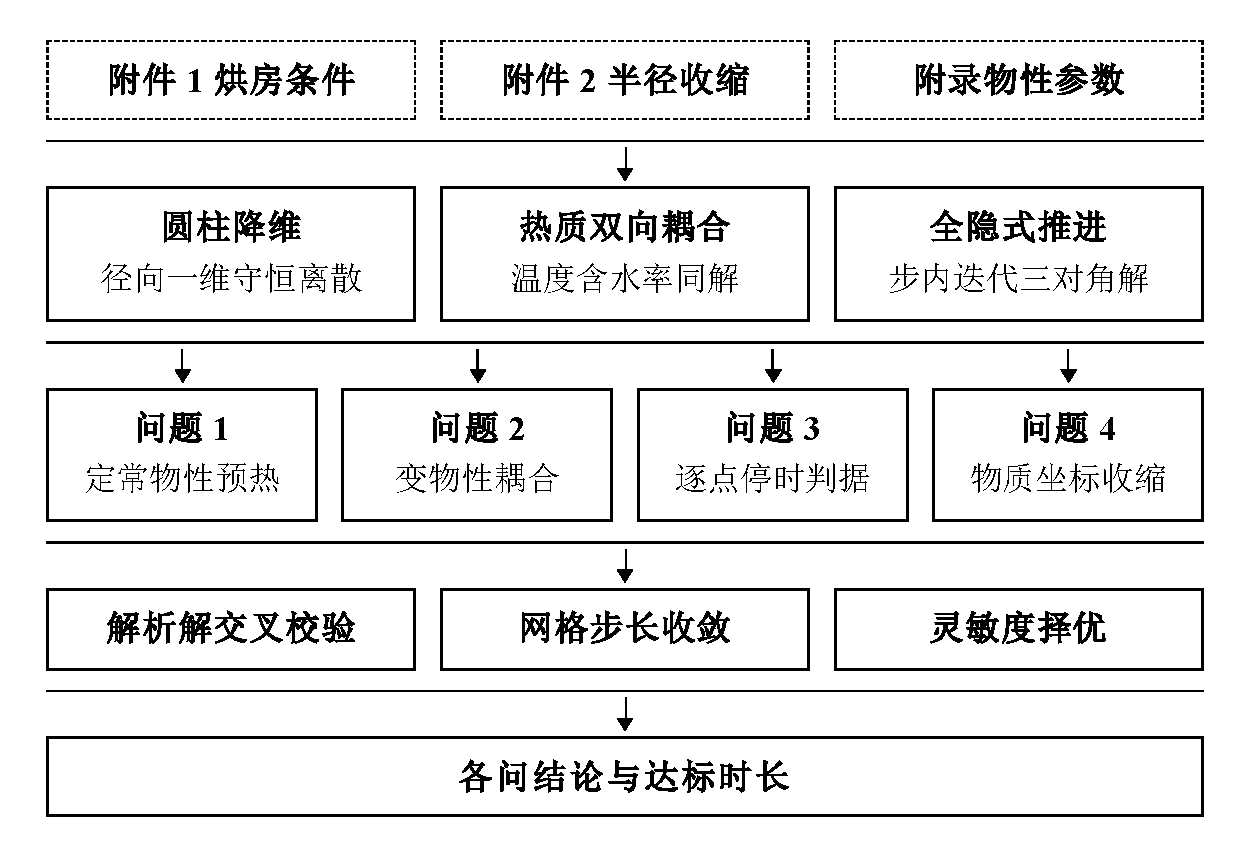
\includegraphics[width=0.8\textwidth,height=0.8\textheight,keepaspectratio]{../figures/fig_roadmap.pdf}
  \caption{全文技术路线。自上而下依次为题给数据、四问共用的数学内核、四个问题
  的分支求解、可信性校验与结论交付五层；虚线框表示题给数据，加粗框为四问共用的
  耦合内核，层间横线表示先汇总再分发；四个问题框内第二行即该问在内核之上新增的
  处理，可见四问同源而分支互不重复。}
  \label{fig:roadmap}
\end{figure}

图中第二层的耦合内核只建立一次，四条分支各自只在其上添加一项处理：问题一固定物性、固定区域，问题二把物性交给解本身决定，问题三在解之上叠加一个首次达标的判定，问题四让区域的外边界随实测半径移动。这种分层使得四问的差异可以被逐项分离，时长变化中的物性效应与几何效应因而各有对应的分支，不必混在一起解释。下面按题目编号说明各问的任务性质与建模取向。

\subsection{问题一的分析}

问题一是一个给定时变边界激励的初边值问题。药材初始温度与含水率均匀，烘房空气的温度与含湿由实测序列给定，需要求出半小时内温度场与水分场沿半径的演化。任务本身并不复杂，难点在于两个场的时间尺度相差悬殊：由该阶段的常物性算得热扩散率约为 $1.69\times10^{-7}$~m$^2$/s，而初始含水率下的水分扩散系数只有约 $4.9\times10^{-9}$~m$^2$/s，相差三十余倍。这意味着半小时之内热量已经能够穿透整个截面，水分却只在表层附近发生可观的变化，两个场必须在同一套时间推进中分别按各自的尺度求解，不能用同一个准稳态近似草率处理。

选择哪一类边界条件是本问的第一个实质判断。以对流换热系数与半径、导热系数构成的传热毕奥数约为 $1.4$，量级为一，既不允许把药材当成温度均匀的集中体，也不允许把表面温度直接取为空气温度，只有第三类边界条件才能同时容纳内部梯度与表面阻力。传质一侧的毕奥数在初始时刻约为 $3$，随着表层变干而迅速增大到千的量级，表明水分迁移由内部扩散控制，这与文献对切片类物料含水率剖面与传质毕奥数关系的分析一致\upcite{rovedo1998biot}。两者合起来决定了模型形式：圆柱坐标下的一维径向守恒方程，表面两个第三类边界，轴线零通量。求解上采用顶点式有限体积离散配合全隐式时间推进，使离散节点正好落在题目要求输出的径向位置上，同时让轴线的零通量在离散层面自动精确满足。本问确立的方程形式、边界处理与离散框架为后三问共用。

\subsection{问题二的分析}

问题二把时间跨度从半小时拉长到两三天，方程形式沿用问题一，但物性改由本阶段的经验公式给出，密度随含水率线性变化，比热容与导热系数随湿基含水率变化，扩散系数则同时含有含水率因子与温度的 Arrhenius 因子。物性一旦依赖待求解，方程就由线性变为非线性，每个时间层都需要用当前解重新计算系数并迭代到自洽，本文为此在每一步内嵌一层不动点迭代。

真正需要小心的是扩散系数的取值位置。经验式中含水率以倒数形式进入指数，表层含水率越过阈值继续下降时扩散系数会跨越四个数量级，相邻两个节点上的取值可能相差十倍以上。此时若沿用常规的算术平均或调和平均来构造控制体界面上的扩散系数，界面通量会被系统性地拉向偏大或偏小的一侧，尤其是调和平均在一侧数值极小时几乎把界面通量压至零，导致失水速率失真。本文改用沿两节点连线对扩散系数作积分平均，使离散通量与扩散势差的关系保持一致。此外经验式中的温度必须取绝对温度，若误用摄氏读数，Arrhenius 因子会被放大若干个数量级。本问输出的全过程解直接作为问题三判定停时的对象。

\subsection{问题三的分析}

问题三不引入新的物理机制，它改变的是提问方式：前两问求场的演化，本问求一个由场定义的时刻。题目要求药材各处的水分浓度都低于阈值，因而合格与否取决于全域中最湿的那一点，而不是表面读数或截面平均值。这三种可能的判据在时间轴上的触发次序是确定的：表面最先达标，截面平均次之，全域最大值最后，若误用前两者会系统性地低估所需时长。轴对称与外向失水的组合使最湿位置始终位于轴线附近，因此判据量在数值上表现为中心含水率，但其定义仍应写成径向最大值，以免在其他工况下失效。

由此本问归结为一个首次穿越时刻的确定：在离散输出的时间序列上逐点比较判据量与阈值，找到符号改变的那一个区间，再在区间内插值定位。由于判据量在阈值附近单调下降且只穿越一次，插值给出的时刻是唯一的。需要一并说明的是，停时是判据量恰好等于阈值的时刻，此刻药材最湿处的含水率等于阈值而非严格小于阈值，严格不等式在其后的任意时刻成立，交付结果的读法需要据此解释。

\subsection{问题四的分析}

问题四新增的是几何：药材因失水而收缩，半径由实测序列给出，求解区域的外边界随时间向轴线移动。前三问在固定区域上写出的方程不再直接适用，处理移动边界有两条路线，一是保留实验室坐标而让网格随边界收缩，二是引入以当前半径归一的物质坐标把区域固定下来，后者是食品与农产品干燥中处理收缩的常用途径\upcite{adrover2018moving,xanthopoulos2026mb}。本文取后者：把半径与当前半径之比作为空间自变量后，网格节点随物质一同向轴线移动，链式法则展开时坐标变换项与表观对流项恰好相消，方程中不再显式出现半径变化率，边界始终落在坐标的端点上。收缩效应则以当前半径平方的倒数进入扩散项，半径缩小意味着同样的含水率落差被压缩在更短的距离上，梯度增大，干燥因此加快。两种写法在数学上是等价的，本文用实验室坐标的写法作为独立对照来交叉检验实现的正确性。

本问时长与问题三的差异有两个来源且方向相反。物性组更换到收缩情形对应的一套后，扩散系数的前因子显著变小，单看这一项会使干燥明显变慢；几何收缩则如上所述使干燥加快。只有把两者分开计算才能说明最终时长为何仍短于问题三。另外，收缩过程中水分不断离开药材而干物质总量应保持不变，这为模型提供了一个不依赖判据的独立检验：干物质的径向积分在整个过程中是否守恒，以及由实测半径反推的干物质密度与经验公式给出的密度是否相容。

\needspace{8\baselineskip}
\section{模型假设}

本文只补充题面未给定而模型必须明确的现实简化，每条假设后附其成立依据。

（1）药材内部的温度与含水率只沿半径变化，轴向与周向的梯度可以忽略。药材长 25~cm、半径 2~cm，侧面积与两端面积之比等于长度与半径之比即 $12.5$，端面换热仅占总表面的 $7.4\%$；题目要求给出的也只是“到药材中心距离”处的结果，径向是题意认定的唯一空间方向。

（2）药材视为均质连续介质，孔隙内水分的整体迁移等效为遵循 Fick 定律的扩散过程，不区分自由水与结合水，也不单独建立气相压力场。题目已直接给出水分浓度扩散系数的经验公式，即指定了本构关系的形式，这种以有效扩散系数概括内部迁移的做法在干燥建模中被广泛采用\upcite{ding2026timevar}；若另建两相多孔介质模型，则需要引入题面未提供的渗透率与毛细压力等参数\upcite{whitaker1977porous}。

（3）能量方程只含导热项与表面对流换热，不设置蒸发相变的源汇项。题目在能量一侧只给出密度、比热容、导热系数与对流换热系数四个参数，三组附录中均无蒸发潜热，故主模型不从常识补入该参数。这一简化的影响本文如实登记而不宣称可忽略：另设一支在热方程中加入潜热汇、潜热取量级参考值 $2.4\times10^6$~J/kg，算得的烘干时长比不设潜热汇的基准慢约一成，即若题目提供潜热数据，结果应向偏慢一侧修正；具体数值见第~\ref{sec:sens} 节的对照算例。

（4）表面对流传质的驱动力取药材表面含水率与烘房空气水分浓度之差。题目对药材写“水分浓度（即干基含水率）”、对烘房同样写“水分浓度”，二者单位相同且只给出一个对流传质系数，无换算系数可用；量纲上传质系数与含水率之积同扩散系数与含水率梯度之积一致，边界条件自洽。

（5）烘房激励在实测序列覆盖的四小时之后按其尾段实测平台值延拓，取空气温度 $49.9989$~°C、空气水分浓度 $0.049988$~kg/kg。题目明示烘干包含预热平衡与恒温干燥两个阶段且全程持续两到三天，实测序列恰好覆盖前一阶段，尾段增量已落在零附近；延拓值取自实测而非拟合外推，不引入题外参数。

（6）问题四中的收缩为径向仿射收缩，轴向长度保持不变，半径随时间的变化完全由实测序列给定。题目要求“根据附件 2”确定时长，即把半径序列定为已知输入；轴向不收缩这一点还得到干物质守恒的独立支持，若改设为各向同性收缩，反推的干物质密度将大幅超出经验公式给出的绝干值。

\section{符号说明}

表~\ref{tab:symbols} 收录全文反复使用、并直接进入控制方程或边界条件的核心记号，其余临时下标与一次性派生量在首次出现处就地说明。

% longtable 自己按 \LTleft/\LTright 居中，不能再套 center：center 是 list 环境，
% 跨页拆分时其无限收缩胶会触发 "Infinite glue shrinkage found in box being split"。
\begin{longtable}{cll}
\caption{核心符号说明}\label{tab:symbols}\\
\toprule
符号 & 含义 & 单位 \\
\midrule
\endfirsthead
\multicolumn{3}{c}{续表~\thetable\quad 核心符号说明}\\
\toprule
符号 & 含义 & 单位 \\
\midrule
\endhead
\bottomrule
\endfoot
$r$ & 径向坐标，自药材中心量起 & m \\
$t$ & 时间 & s \\
$R_0$ & 药材初始半径 & m \\
$R(t)$ & 问题四中随时间收缩的当前半径 & m \\
$s$ & 物质径向坐标，$s=r/R(t)$ & --- \\
$T(r,t)$ & 药材温度 & °C \\
$T_{\rm K}$ & 药材绝对温度，$T_{\rm K}=T+273.15$ & K \\
$C(r,t)$ & 药材干基含水率 & kg/kg \\
$T_a(t)$ & 烘房空气温度 & °C \\
$C_a(t)$ & 烘房空气水分浓度 & kg/kg \\
$\rho(C)$ & 药材湿基密度 & kg/m$^3$ \\
$\rho_{\rm d}$ & 干物质密度，$\rho_{\rm d}=\rho/(1+C)$ & kg/m$^3$ \\
$c_p(C)$ & 药材比热容 & J/(kg$\cdot$K) \\
$\lambda(C)$ & 药材热传导系数 & W/(m$\cdot$K) \\
$D(C,T)$ & 水分浓度扩散系数 & m$^2$/s \\
$h$ & 对流换热系数 & W/(m$^2\cdot$K) \\
$h_m$ & 对流传质系数 & m/s \\
$C_{\rm th}$ & 烘干合格的含水率阈值 & kg/kg \\
$t_{\rm dry}$ & 烘干所需时间 & h \\
${\rm Bi}_h,\ {\rm Bi}_m$ & 传热与传质毕奥数，$hR/\lambda$ 与 $h_mR/D$ & --- \\
\end{longtable}

\section{耦合传热传质的公共建模框架}

四个问题共用同一套守恒律、同一种边界条件形式和同一个求解器，差别只在物性库、求解区域与终止条件。本节一次性建立公共部分，各问章节只说明保留了什么、新增了什么以及结果因此改变了什么。

\subsection{几何降维与控制方程}

药材是一段长 25~cm、半径 2~cm 的圆柱。侧面积与两端面积之比等于长度与半径之比，端面只占总换热面积的 $7.4\%$，加之题目要求的结果都以“到药材中心的距离”标定，因此把三维圆柱问题降为一维径向问题。降维之后表面只剩一个环柱面，它同时承担对流换热与对流传质两个交换过程，轴线则由对称性给出零通量。图~\ref{fig:mech-geometry} 把这一降维过程与三处边界的类型画在一起。

\begin{figure}[htbp]
  \centering
  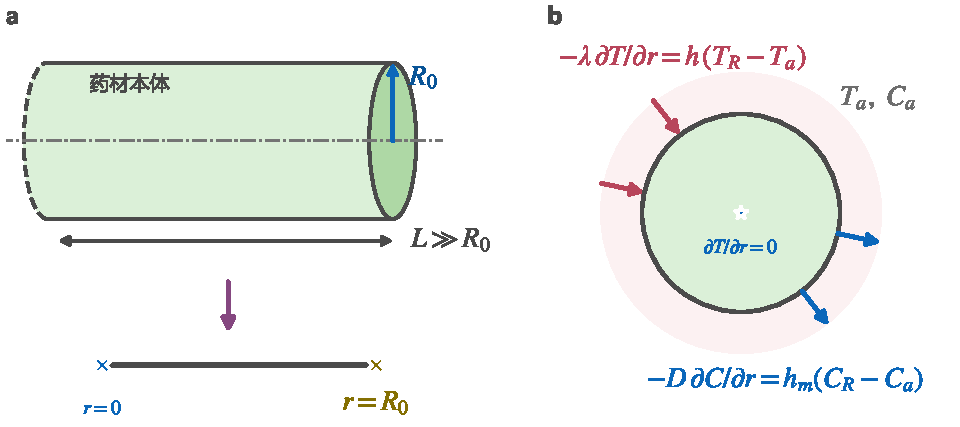
\includegraphics[width=0.9\textwidth,height=0.8\textheight,keepaspectratio]{../figures/fig_mech_geometry.pdf}
  \caption{几何降维与边界条件。长径比足够大时轴向与周向梯度可略，三维圆柱
  问题降为一维径向问题；表面同时承担对流换热与对流传质两个 Robin 条件，
  轴线处由对称性给出零通量。}
  \label{fig:mech-geometry}
\end{figure}

图中表面处两个箭头方向相反：热量向内输入，水分向外输出，两者共用同一张表面却由两个独立的传递系数控制。轴线处没有箭头，它不是一个物理壁面而是对称面，这一点在离散时会带来便利。

在此几何下取以轴线为轴、半径 $r$、厚 $\mathrm{d}r$ 的环形控制体。能量守恒要求控制体内能的增率等于两个柱面净导入的热流，写成

\begin{equation}
\frac{\partial}{\partial t}\Big[\rho(C)c_p(C)\,T\Big]\cdot 2\pi r\,\mathrm{d}r
= -\frac{\partial}{\partial r}\Big[2\pi r\,q\Big]\mathrm{d}r,
\qquad q=-\lambda(C)\frac{\partial T}{\partial r},
\label{eq:econs}
\end{equation}

其中 $q$ 是 Fourier 定律给出的径向热流密度。水分一侧以干物质为参照计量，同样的守恒论证给出

\begin{equation}
\frac{\partial C}{\partial t}\cdot 2\pi r\,\mathrm{d}r
=-\frac{\partial}{\partial r}\Big[2\pi r\,j\Big]\mathrm{d}r,
\qquad j=-D(C,T)\frac{\partial C}{\partial r},
\label{eq:mcons}
\end{equation}

$j$ 为 Fick 定律给出的水分通量。由于含水率以“千克水每千克干物质”计量，$j$ 的量纲为 m/s。整理式~\eqref{eq:econs} 与式~\eqref{eq:mcons}，得到四问共用的控制方程

\begin{equation}
\rho(C)\,c_p(C)\,\frac{\partial T}{\partial t}
=\frac{1}{r}\frac{\partial}{\partial r}\!\left(r\,\lambda(C)\frac{\partial T}{\partial r}\right),
\label{eq:heat}
\end{equation}

\begin{equation}
\frac{\partial C}{\partial t}
=\frac{1}{r}\frac{\partial}{\partial r}\!\left(r\,D(C,T)\frac{\partial C}{\partial r}\right).
\label{eq:mass}
\end{equation}

两式中的 $1/r$ 与 $r$ 加权因子来自圆柱几何的面积增长，这是本题区别于平板问题的根本之处。题目所给附录只提供了 $\rho(C)$ 与 $c_p(C)$ 的代数关系而未给出能量的守恒形式，故式~\eqref{eq:heat} 按附录的写法把 $\rho c_p$ 置于时间导数之外，不额外引入题面未定义的 $\partial(\rho c_p)/\partial t$ 项。图~\ref{fig:mech-coupling} 给出面积加权项的来源与两个方程之间的耦合关系。

\begin{figure}[htbp]
  \centering
  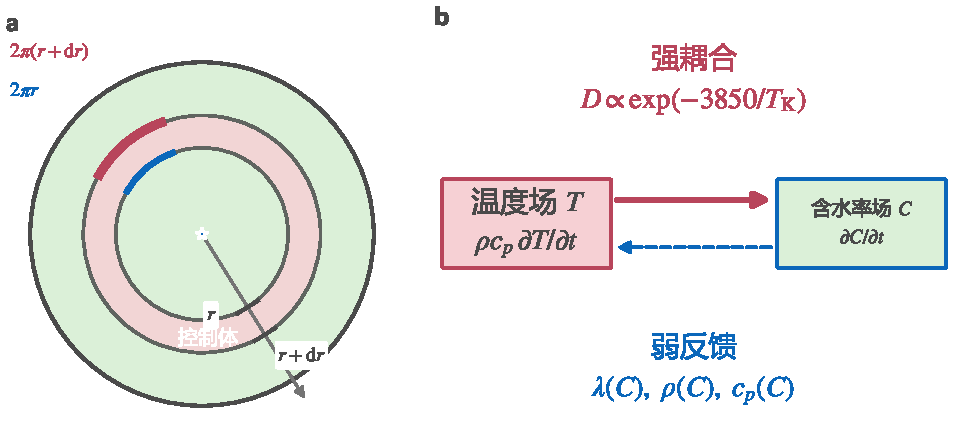
\includegraphics[width=0.9\textwidth,height=0.8\textheight,keepaspectratio]{../figures/fig_mech_coupling.pdf}
  \caption{守恒律的面积加权与双向耦合。环形控制体内外两个柱面的通过面积不
  相等，这是圆柱几何区别于平板的根源，整理后在方程中留下面积加权项；温度对
  扩散系数是强耦合，含水率对热物性只是弱反馈。}
  \label{fig:mech-coupling}
\end{figure}

左侧图示说明同样大小的通量在大半径处对应更大的通过面积，因此表面附近的浓度变化被放大而中心区被相对屏蔽；干燥总是从外向内推进，几何本身已经贡献了一部分原因。右侧则表明两个方程的耦合是不对称的：温度经 Arrhenius 因子强烈改变扩散系数，含水率只通过密度、比热容与导热系数对温度场的时间常数产生温和的反馈。这种单向强、反向弱的结构使得求解时可以把两个方程放在同一时间层内迭代，而不必担心反馈回路造成的迭代震荡。

\subsection{初始条件、边界条件与烘房激励}

初始时刻药材整体处于均匀状态，

\begin{equation}
T(r,0)=T_0=28\ ^{\circ}\mathrm{C},\qquad C(r,0)=C_0=2.55\ \mathrm{kg/kg},\qquad 0\le r\le R_0 .
\label{eq:ic}
\end{equation}

轴线处由轴对称性给出零通量，

\begin{equation}
\left.\frac{\partial T}{\partial r}\right|_{r=0}=0,\qquad
\left.\frac{\partial C}{\partial r}\right|_{r=0}=0 .
\label{eq:bc0}
\end{equation}

表面处热量与水分都以第三类边界条件与烘房交换，即内部输运到表面的通量等于表面与空气之间的对流交换量，

\begin{equation}
\left.-\lambda(C)\frac{\partial T}{\partial r}\right|_{r=R}=h\,\big[T(R,t)-T_a(t)\big],
\qquad
\left.-D(C,T)\frac{\partial C}{\partial r}\right|_{r=R}=h_m\,\big[C(R,t)-C_a(t)\big].
\label{eq:bcR}
\end{equation}

题目给出的对流换热系数 $25$~W/(m$^2\cdot$K) 与热风干燥实测的对流换热系数量级相符\upcite{akpinar2015htc}，而只给一个对流传质系数、不给相间换算关系的做法，与传热传质类比中以同一形式处理两个 Robin 条件的惯例一致\upcite{ghiaasiaan2018analogy}。选择第三类而非第一类边界并非形式偏好。以初始物性估算，传热毕奥数 ${\rm Bi}_h=hR_0/\lambda\approx1.4$，量级为一，说明表面对流阻力与内部导热阻力相当，既不能把药材当作温度均匀的集中体，也不能把表面温度直接指定为空气温度。传质一侧 ${\rm Bi}_m=h_mR_0/D$ 在初始时刻约为 $3$，随着表层变干而增大到千的量级，表明水分迁移越来越受内部扩散控制，表面对流则退化为一个次要环节。

需要强调，式~\eqref{eq:bcR} 中的 $C$ 与 $C_a$ 虽同为“水分浓度”且单位相同，却分属药材与空气两个载体，数值上相差约两个数量级，任何环节都不得把两者合并为同一个场。烘房激励 $T_a(t)$ 与 $C_a(t)$ 由实测序列线性插值给出，图~\ref{fig:oven-input} 展示了这套激励的形态及其延拓依据。

\begin{figure}[htbp]
  \centering
  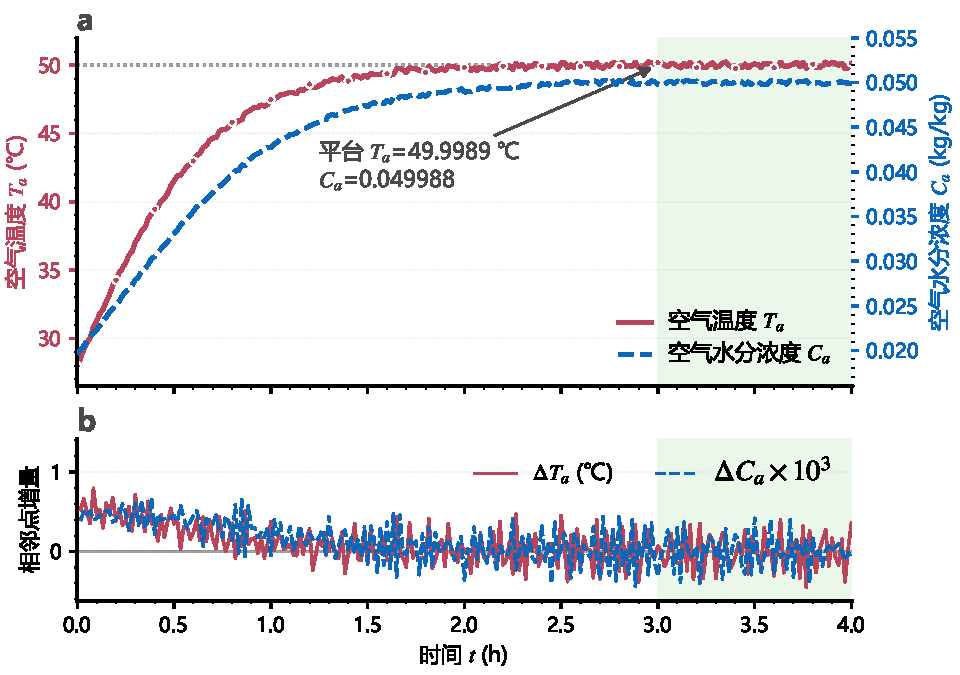
\includegraphics[width=0.9\textwidth,height=0.8\textheight,keepaspectratio]{../figures/fig_oven_input.pdf}
  \caption{附件 1 给出的烘房运行条件（241 点实测，未作平滑）。a：空气温度
  $T_a$ 先升温后维持恒定，空气水分浓度 $C_a$ 与之反向变化，两者是表面两个
  Robin 边界的驱动量；b：逐点一阶差分，末段 61 点的增量落在零线附近，据此
  判定序列已进入恒定平台，平台均值用于时间超出实测区间后的延拓。}
  \label{fig:oven-input}
\end{figure}

实测序列在四小时内把空气温度由 $28$~°C 抬到约 $50$~°C 后保持不动，空气水分浓度则由 $0.0196$~kg/kg 升到约 $0.0500$~kg/kg，两者反向变化对应加热与加湿的先后。右图的逐点差分把“是否已进入平台”变成一个可判断的问题：末段 61 个点的增量全部贴近零线，因此把该段的实测均值 $T_a=49.9989$~°C、$C_a=0.049988$~kg/kg 用作四小时之后的常值延拓，而不是对趋势作外推拟合。这样处理的代价是全程约九成的时间依赖平台假设，好处是不引入题面之外的任何参数。

\subsection{三套物性及其适用范围}

题目为三个不同情形分别给出物性经验公式，且互相排斥：预热阶段用第一套，全过程与合格时长判定用第二套，考虑收缩时用第三套；对流换热系数 $h=25$~W/(m$^2\cdot$K) 与对流传质系数 $h_m=8\times10^{-7}$~m/s 则全题通用。三套物性的具体形式为
\begin{align}
\text{附录 2：}&\ \rho=820,\quad c_p=2600,\quad \lambda=0.36,\quad D=7\times10^{-9}e^{-0.89/C};
\label{eq:app2}\\
\text{附录 3：}&\ \rho=650+128C,\quad c_p=1450+2736\tfrac{C}{C+1},\quad
\lambda=0.21+0.38\tfrac{C}{C+1},\notag\\
&\ D=2.4\times10^{-3}e^{-0.45/C}e^{-3850/T_{\rm K}};
\label{eq:app3}\\
\text{附录 4：}&\ \rho=760+90C,\quad c_p=1850+2150\tfrac{C}{C+1},\quad
\lambda=0.12+0.20\tfrac{C}{C+1},\notag\\
&\ D=4.2\times10^{-4}e^{-0.30/C}e^{-3850/T_{\rm K}} .
\label{eq:app4}
\end{align}

三套物性中扩散系数同时含有含水率因子与温度因子，这与实验测定给出的有效扩散系数形式一致：温度依赖按 Arrhenius 型给出\upcite{doymaz2016kinetics}，含水率依赖则来自内部迁移阻力随脱水而变化\upcite{yang2007internal}，两者相乘的写法在不同干燥方式的实测数据上都能成立\upcite{richter2016vacuum}。三处细节直接决定结果是否正确。其一，Arrhenius 因子中的温度必须取绝对温度，若误用摄氏读数，指数项将相差数十个数量级，干燥过程永远不会结束。其二，浓度因子的指数为 $-a/C$，含水率在分母上，因此扩散系数随药材变干而减小，这正是干燥后期表层阻力急剧增大、也就是俗称“结壳”的数学表现。其三，比热容与导热系数的自变量是湿基含水率 $C/(C{+}1)$ 而非干基含水率，初始状态下前者为 $0.7183$，若误用干基会使两项系统性偏大。图~\ref{fig:prop-curves} 把三套物性逐项画在一起。

\begin{figure}[htbp]
  \centering
  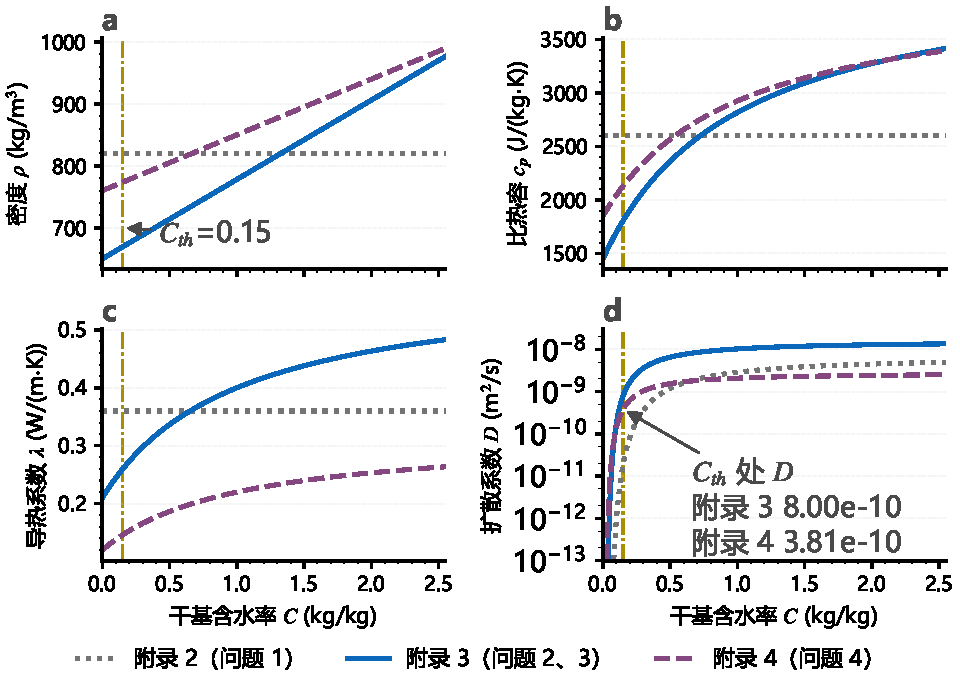
\includegraphics[width=0.9\textwidth,height=0.8\textheight,keepaspectratio]{../figures/fig_prop_curves.pdf}
  \caption{附录 2/3/4 三套物性的逐项对照，横轴为干基含水率，点划线标出判据
  阈值 $C_{th}=0.15$ 的位置。a—c：密度、比热容、导热系数；附录 2 为常物性，
  附录 3/4 随含水率变化（比热与导热按湿基 $C/(C{+}1)$ 取值）。d：扩散系数取
  对数纵轴，跨越四个数量级，是三套物性中差异最大的一项。曲线均按附录给出的
  经验公式直接计算，未作任何拟合或平滑。}
  \label{fig:prop-curves}
\end{figure}

前三幅图中，密度、比热容与导热系数在整个含水率区间内的变化都不超过一倍，其中导热系数从湿态的 $0.48$ 降到阈值附近的 $0.26$，量级始终不变。第四幅图必须用对数纵轴才能容纳：第二套物性在 $50$~°C 下，扩散系数由初始含水率处的 $1.35\times10^{-8}$~m$^2$/s 降到阈值处的 $8.0\times10^{-10}$~m$^2$/s，再降到最干处的 $2.0\times10^{-12}$~m$^2$/s，前后跨越四个数量级。这一项既是数值求解全部困难的来源，也是三套物性中差异最大的一项——第三套的前因子比第二套小了将近一个数量级。

\subsection{顶点式有限体积离散}

物性随解变化使方程为非线性，且扩散系数在空间上的刚性比可达 $10^4$，离散格式必须同时保证守恒性与稳定性。本文采用顶点式有限体积法：把归一化半径 $N$ 等分，节点取在 $s_i=i\Delta s$，$\Delta s=1/N$，控制体取相邻节点的中点连线所夹区间，两端为半控制体。选顶点式而非格心式的直接理由是题目要求的输出位置恰好落在节点上，$N=20$ 时节点即 $r=0,0.1,\dots,2.0$~cm，加密到 $N=40$ 或 $80$ 时原节点仍是子集，交付结果无需任何空间插值。控制体的无量纲体积由精确积分得到，

\begin{equation}
V_0=\frac{(\Delta s)^2}{8},\qquad
V_i=i\,(\Delta s)^2\ (1\le i\le N-1),\qquad
V_N=\frac{(\Delta s)^2}{2}\left(N-\frac14\right),
\label{eq:vol}
\end{equation}

三式合起来满足 $\sum_i V_i=1/2=\int_0^1 s\,\mathrm{d}s$，即离散域的体积与连续域严格相等。把式~\eqref{eq:mass} 在控制体上积分，散度项化为界面通量之差，得

\begin{equation}
V_i\frac{C_i^{n+1}-C_i^{n}}{\Delta t}
=\frac{1}{R^2}\left[
s_{i+\frac12}D_{i+\frac12}\frac{C_{i+1}^{n+1}-C_i^{n+1}}{\Delta s}
-s_{i-\frac12}D_{i-\frac12}\frac{C_i^{n+1}-C_{i-1}^{n+1}}{\Delta s}\right].
\label{eq:disc}
\end{equation}

两个边界都不需要虚节点。轴线一侧的界面面积因子 $s_{-1/2}=0$ 使该项自动消失，式~\eqref{eq:bc0} 的零通量条件在离散层面精确满足；表面一侧的界面就是物理表面，把式~\eqref{eq:bcR} 直接代入即贡献一项 $-h_m\big[C_N^{n+1}-C_a\big]/R$。温度方程与之同构，只需把 $V_i$ 换成 $\rho_ic_{p,i}V_i$、$D$ 换成 $\lambda$、$h_m$ 换成 $h$、$C_a$ 换成 $T_a$。图~\ref{fig:mech-fvm} 给出网格布置与由此得到的代数结构。

\begin{figure}[htbp]
  \centering
  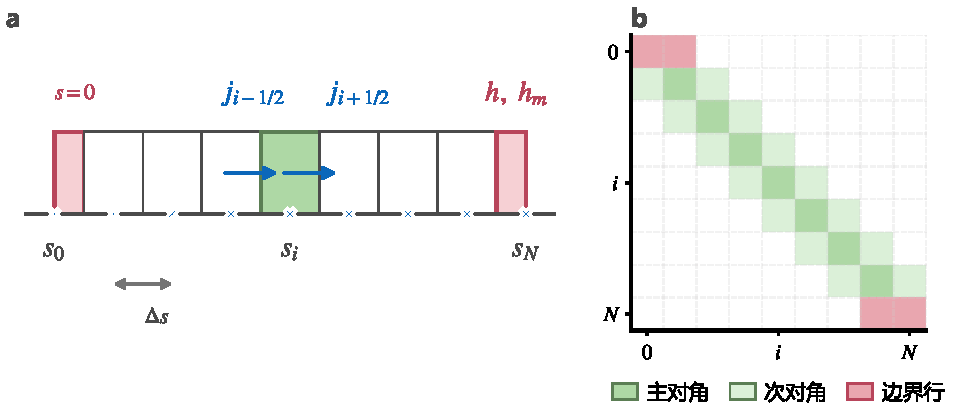
\includegraphics[width=0.9\textwidth,height=0.8\textheight,keepaspectratio]{../figures/fig_mech_fvm.pdf}
  \caption{顶点式有限体积网格与代数结构。节点落在输出要求的位置上，两端为
  半控制体；内侧界面的面积因子为零使轴线零通量精确满足，不需虚节点，由此得
  到的系数矩阵严格三对角。图中网格数仅为作图清晰，不代表实算网格。}
  \label{fig:mech-fvm}
\end{figure}

由于每个控制体只与左右两个邻居交换通量，系数矩阵严格三对角，可用追赶法在 $O(N)$ 次运算内直接求解，不引入迭代求逆的误差。时间方向采用全隐式格式：显式格式的稳定性上限为 $\Delta t\le\Delta r^2/(2D_{\max})$，本题扩散系数的空间最大值出现在湿润的中心区，在 $\Delta r=5\times10^{-4}$~m 时该上限约为 $9.3$~s，而总时长在 $2\times10^5$~s 量级，显式推进需要数万步且步长完全由稳定性而非精度决定。全隐式配合三对角直接解使时间步只受精度约束。

\subsection{界面扩散系数的取法}

式~\eqref{eq:disc} 中界面系数 $D_{i+1/2}$ 的取法在本题中不是细节。扩散系数跨越四个数量级，相邻节点上的取值可能相差十倍以上，此时常用的调和平均会被两者中的较小者支配，$D_{i+1/2}\approx2\min(D_i,D_{i+1})$。表面附近含水率梯度极陡，最外侧控制体的含水率随网格加密而不断降低，界面系数随之持续变小，形成不随网格细化而消失的偏差。实算可以直接看到这一失效：取调和平均时，$N=20,40,80$ 给出的合格时长为 $549.918$、$223.428$、$87.440$~h，网格每加倍结果几近减半，根本不收敛。

问题的根源在于调和平均的适用前提是界面两侧为分区常系数的复合介质，此时串联阻力叠加给出精确通量；而本题的 $D(C,T)$ 是含水率的光滑函数，界面两侧的差异完全由离散产生，并非物理跳变。回到通量本身即可得到正确的取法：引入 Kirchhoff 势 $\Phi(C)=\int_0^C D(c,\bar T)\,\mathrm{d}c$ 后通量写作 $j=-\partial\Phi/\partial r$，相邻节点间的精确通量为 $-(\Phi_{i+1}-\Phi_i)/\Delta r$。把它整理成式~\eqref{eq:disc} 所用的形式，界面系数只能是

\begin{equation}
D_{i+\frac12}=\frac{1}{C_{i+1}-C_i}\int_{C_i}^{C_{i+1}} D\!\left(c,\ \tfrac{T_i+T_{i+1}}{2}\right)\mathrm{d}c ,
\qquad
\lim_{C_{i+1}\to C_i}D_{i+\frac12}=D\!\left(C_i,\tfrac{T_i+T_{i+1}}{2}\right).
\label{eq:iface}
\end{equation}

该积分用八点 Gauss--Legendre 求积计算，对 $e^{-a/C}$ 型被积函数的相对误差在 $10^{-10}$ 以下；两节点含水率之差小于 $10^{-12}$ 时退化为中点取值以避免零比零。改用积分平均后，同一组网格给出的合格时长立即收敛，逐档变化只有 $0.052\%$ 与 $0.014\%$，不再有随网格漂移的趋势；三档的具体数值列于表~\ref{tab:conv}。式~\eqref{eq:iface} 在系数为常数时退化为该常数，在真实分区跳变时退化为调和平均，因此是算术平均与调和平均的共同推广，没有适用性损失。导热系数在整个区间内变化不足一倍，其界面取值方式对结果无实质影响，仍按调和平均处理。

\subsection{非线性迭代与时间步安排}

物性依赖待求解，故每个时间层内做一轮不动点迭代：以上一层解为初值，用当前迭代值计算 $\rho,c_p,\lambda,D$ 与界面系数，解两个三对角系统，直到

\begin{equation}
\max\!\Big(\big\|C^{(k+1)}-C^{(k)}\big\|_\infty,\ \ 10^{-3}\big\|T^{(k+1)}-T^{(k)}\big\|_\infty\Big)<10^{-11},
\label{eq:picard}
\end{equation}

迭代次数上限取 60。式~\eqref{eq:picard} 中温度残差乘以 $10^{-3}$ 是一个容差配比：两个场的单位不同，用同一个绝对阈值并无意义，该权因子相当于对含水率要求 $10^{-11}$~kg/kg、对温度要求 $10^{-8}$~°C。含水率一侧收得更紧是因为停时判据直接由含水率定义，而 $10^{-8}$~°C 的温度残差已远低于任何有物理意义的分辨率。实算表明恒温平台段三到五次迭代即收敛，预热段峰值为 12 次。

时间步按阶段分段：$1800$~s 以内取 $0.01$~s 以分辨升温初期最陡的瞬变，$1800$ 至 $14400$~s 取 $1$~s 覆盖实测激励段，其后取 $60$~s 与后续输出间隔一致。各问的输出间隔按题面要求另行设定（问题一、二每 $1$~s，问题三、四每 $60$~s），都是相应步长的整数倍，逐秒输出的要求由此自动满足。平台段的步长收敛性经实算确认：$\Delta t$ 由 $120$~s 依次细化到 $60$、$30$、$10$~s，合格时长的逐档相对变化为 $0.081\%$、$0.041\%$、$0.027\%$，$60$~s 相对 $10$~s 的偏差为 $0.068\%$，已远小于结果的有效位数需求，因此取 $60$~s 作为生产设置；四档数值同见表~\ref{tab:conv}。

\section{问题一：预热平衡阶段的常物性耦合场模型}

\subsection{模型的具体化}

预热阶段采用附录 2 给出的一组参数，即式~\eqref{eq:app2}：密度、比热容与导热系数取常值，扩散系数只依赖含水率。把它代入公共框架式~\eqref{eq:heat}--\eqref{eq:mass}，热方程的系数不再随解变化，退化为常系数线性方程

\begin{equation}
\frac{\partial T}{\partial t}=\alpha\left(\frac{\partial^2 T}{\partial r^2}+\frac{1}{r}\frac{\partial T}{\partial r}\right),
\qquad
\alpha=\frac{\lambda}{\rho c_p}=\frac{0.36}{820\times2600}=1.6886\times10^{-7}\ \mathrm{m^2/s},
\label{eq:q1alpha}
\end{equation}

水分方程则仍是非线性的，因为扩散系数含 $e^{-0.89/C}$。初始条件按式~\eqref{eq:ic} 取均匀分布。以 $\alpha$ 与初始含水率处的扩散系数 $D(C_0)=4.938\times10^{-9}$~m$^2$/s 分别估算特征时间：热扩散的 $R_0^2/\alpha\approx2.37\times10^3$~s，水分扩散的 $R_0^2/D\approx8.1\times10^4$~s。半小时的观测窗恰好覆盖前者而远短于后者，这就预告了本阶段的基本图景——温度已能贯穿整个截面，水分只在表层附近发生变化。传热毕奥数 ${\rm Bi}_h=1.3889$、初始传质毕奥数 ${\rm Bi}_m=3.2404$，两者都远离集中参数模型的适用范围，径向分布必须保留。

\subsection{求解流程}

本问的求解沿公共框架执行，但因物性为常值而不需要非线性迭代，流程相对简明，如图~\ref{fig:flow-q1}。

\begin{figure}[htbp]
  \centering
  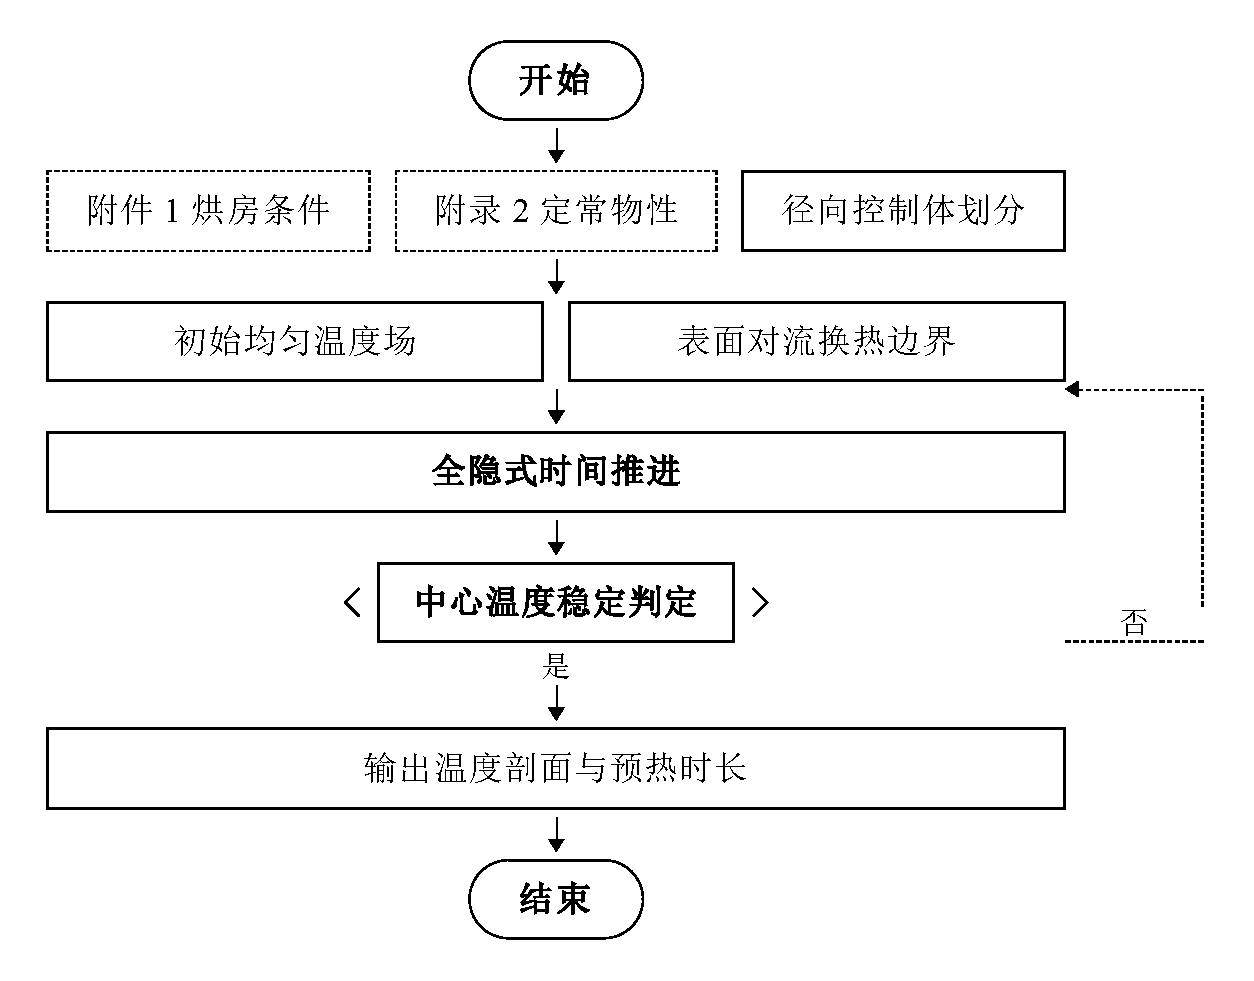
\includegraphics[width=0.8\textwidth,height=0.8\textheight,keepaspectratio]{../figures/fig_flow_q1.pdf}
  \caption{问题 1 的求解流程。自上而下为数据与网格准备、初始与边界设定、全隐式
  时间推进三段，虚线框表示题给数据，加粗框为主控步骤；右侧虚线回路表示中心温度
  未达稳定时返回继续推进，达稳定后输出温度剖面与预热时长。}
  \label{fig:flow-q1}
\end{figure}

流程的三段划分对应三类不同性质的工作：第一段把实测激励和输出网格准备好，网格取 $N=40$ 使节点覆盖全部要求输出的径向位置；第二段把初始条件与两个边界条件装配进系数矩阵；第三段逐步推进并在每步输出。右侧回路的判断依据是中心温度是否仍在明显上升，它决定推进何时终止，而不改变每一步的计算内容。时间步在本问取 $0.01$~s，远小于精度需要，目的是让逐秒输出的结果不受时间离散影响。

\subsection{温度场与水分场的结果}

按题目要求的时刻与位置，温度结果列于表~\ref{tab:q1T}。

\begin{table}[H]
\centering
\caption{30 分钟内药材的温度（单位：°C）}\label{tab:q1T}
\begin{tabular}{cccccc}
\toprule
\multirow{2}{*}{时间/s} & \multicolumn{5}{c}{到药材中心的距离/cm}\\
\cmidrule(lr){2-6}
 & 0 & 0.5 & 1 & 1.5 & 2 \\
\midrule
100  & 28.0001 & 28.0004 & 28.0041 & 28.0327 & 28.1797 \\
300  & 28.0409 & 28.0636 & 28.1514 & 28.3680 & 28.8484 \\
600  & 28.4534 & 28.5361 & 28.8039 & 29.3158 & 30.1649 \\
900  & 29.3244 & 29.4583 & 29.8754 & 30.6160 & 31.7302 \\
1200 & 30.5428 & 30.7098 & 31.2223 & 32.1125 & 33.4275 \\
1500 & 31.9957 & 32.1867 & 32.7660 & 33.7462 & 35.1203 \\
1800 & 33.5753 & 33.7720 & 34.3641 & 35.3621 & 36.7855 \\
\bottomrule
\end{tabular}
\end{table}

表中每一列自上而下都在单调上升，最右列的升幅始终大于最左列，可见升温由表面驱动。同一批时刻与位置上的含水率结果列于表~\ref{tab:q1C}。

\begin{table}[H]
\centering
\caption{30 分钟内药材的水分浓度（单位：kg/kg）}\label{tab:q1C}
\begin{tabular}{cccccc}
\toprule
\multirow{2}{*}{时间/s} & \multicolumn{5}{c}{到药材中心的距离/cm}\\
\cmidrule(lr){2-6}
 & 0 & 0.5 & 1 & 1.5 & 2 \\
\midrule
100  & 2.5500 & 2.5500 & 2.5500 & 2.5500 & 2.2551 \\
300  & 2.5500 & 2.5500 & 2.5500 & 2.5490 & 2.0543 \\
600  & 2.5500 & 2.5500 & 2.5500 & 2.5350 & 1.8788 \\
900  & 2.5500 & 2.5500 & 2.5496 & 2.5044 & 1.7560 \\
1200 & 2.5500 & 2.5500 & 2.5481 & 2.4646 & 1.6595 \\
1500 & 2.5500 & 2.5499 & 2.5444 & 2.4208 & 1.5794 \\
1800 & 2.5500 & 2.5497 & 2.5381 & 2.3757 & 1.5108 \\
\bottomrule
\end{tabular}
\end{table}

两张表呈现出完全不同的节奏。温度方面，半小时内中心由 $28.0000$ 升到 $33.5753$~°C、表面升到 $36.7855$~°C，中心与表面之差始终维持在 $3.2$~°C 左右且各点均在上升，说明热波已经穿透整个截面。含水率方面，表面由 $2.5500$ 降到 $1.5108$~kg/kg，降幅超过四成；而 $r=1$~cm 处仅降到 $2.5381$，中心在四位小数下与初值没有区别。把整个截面平均，含水率由 $2.5500$ 降到 $2.2932$~kg/kg，也就是说这半小时排出的水分几乎全部来自最外侧一层。图~\ref{fig:q1-profiles} 把七个时刻的径向剖面叠在一起。

\begin{figure}[htbp]
  \centering
  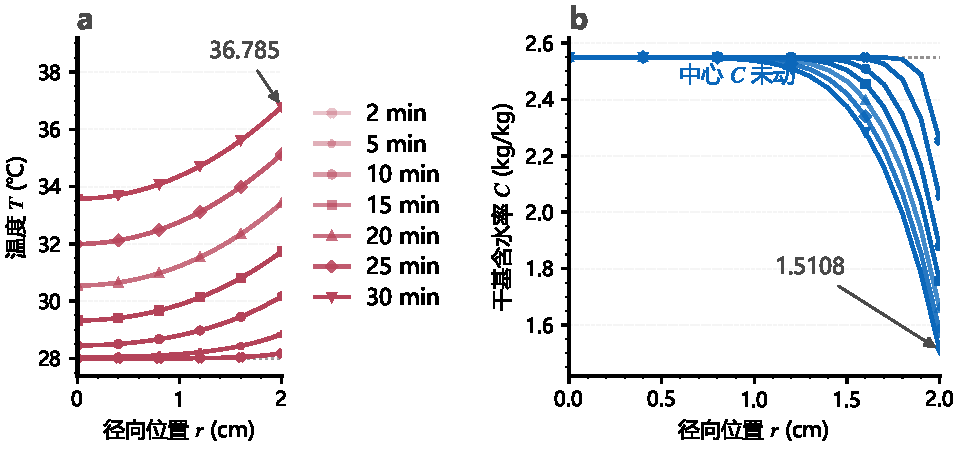
\includegraphics[width=0.9\textwidth,height=0.8\textheight,keepaspectratio]{../figures/fig_q1_profiles.pdf}
  \caption{预热阶段的径向剖面族，7 个输出时刻用同族深浅渐变区分，径向取 21
  个位置（0.1\,cm 间隔）。a：温度剖面自初始均匀态由外向内抬升，表面始终领先
  于中心，中心的追赶速度决定预热时长；b：同期含水率剖面只有表层下降，中心在
  30\,min 内几乎未动，这一快慢分离说明预热段可只看温度判平衡。}
  \label{fig:q1-profiles}
\end{figure}

左图的七条温度剖面整体向上平移而形状变化不大，剖面在表面附近的斜率始终有限，这是第三类边界条件的直接表现：表面温度没有跳到空气温度，而是被对流阻力拖在后面。右图的七条含水率剖面则几乎重合于一条水平线，只在最右端急剧下垂，下垂区宽度约 $0.5$~cm 且随时间缓慢内移。两幅图并置说明，预热阶段判断“是否已经平衡”只需看温度，因为水分场此时尚未真正启动。

把同样的数据换成时间与半径的二维分布，可以更直接地读出两个场的推进速度，见图~\ref{fig:q1-hovmoller}。

\begin{figure}[htbp]
  \centering
  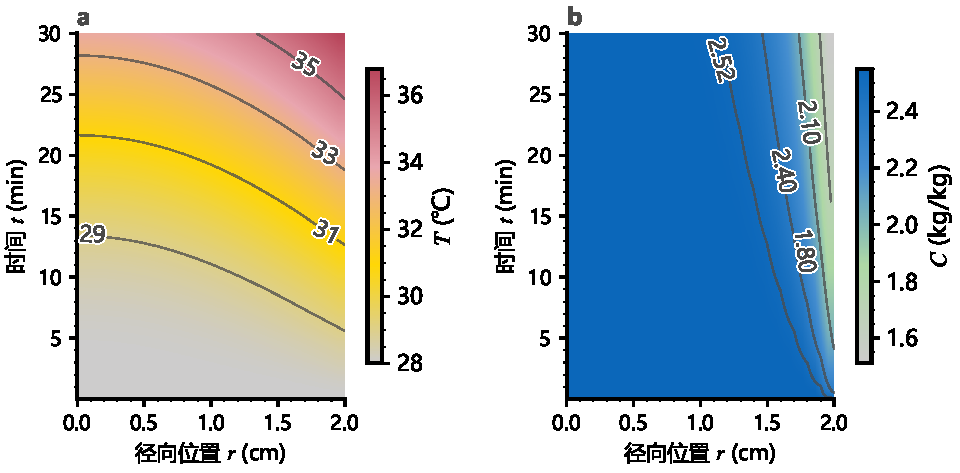
\includegraphics[width=0.9\textwidth,height=0.8\textheight,keepaspectratio]{../figures/fig_q1_hovmoller.pdf}
  \caption{预热阶段温度场与水分场的时间—半径分布（$200\times21$ 输出网格）。
  a：温度等值线自表面向轴线推进，可读出热波到达轴线的时刻与其后的整体抬升；
  b：同期水分场，等值线几乎平行于时间轴，说明 30\,min 内水分尚未形成贯穿性
  梯度。两幅同尺度并置，用于对比热扩散与质扩散的时间尺度差异。}
  \label{fig:q1-hovmoller}
\end{figure}

温度一侧的等值线呈斜向左上的族，每条等值线与纵轴相交的时刻即该温度到达轴线的时刻，可见 $28.5$~°C 的扰动在约 $600$~s 抵达中心，其后各条等值线间距逐渐拉开，反映升温速率随空气温差缩小而放缓。水分一侧的等值线几乎与时间轴平行，全部拥挤在图的右侧边缘，半小时内没有任何一条到达轴线。这两幅图给出的时间尺度比与式~\eqref{eq:q1alpha} 下方由特征时间估算的三十余倍是一致的。

表面通量的演化还揭示了一个不那么直观的现象，见图~\ref{fig:q1-flux}。

\begin{figure}[htbp]
  \centering
  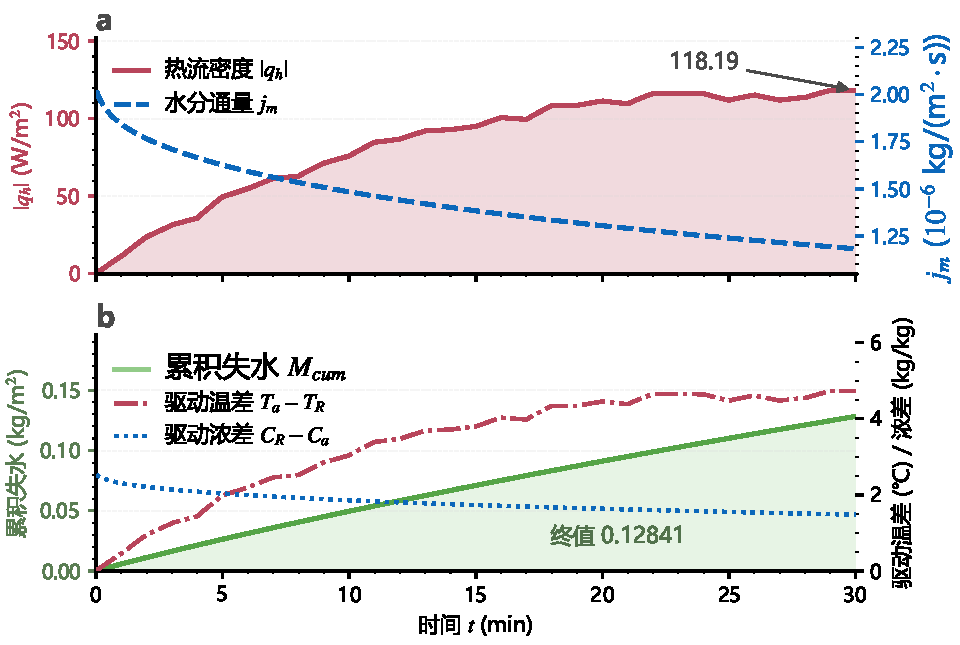
\includegraphics[width=0.9\textwidth,height=0.8\textheight,keepaspectratio]{../figures/fig_q1_flux.pdf}
  \caption{预热阶段表面通量与累积失水（1\,s 输出，1800 点）。a：热流密度
  $|q_h|$ 随表面与空气温差缩小而单调衰减，水分通量 $j_m$ 反而上升，因表面
  升温抬高了平衡含湿的差值；b：累积失水量与两个驱动力（温差、浓差）的同步
  演化，驱动温差衰减而驱动浓差近似持平，故失水近似线性累积。}
  \label{fig:q1-flux}
\end{figure}

热流与水分通量的走向相反：表面热流随着表面温度追近空气温度而单调衰减，水分通量却在同期上升。原因在于两个驱动力的变化方向不同，表面与空气的温差在缩小，而表面含水率与空气水分浓度之差在整个半小时内基本维持，于是累积失水量近似线性增长。这一对照说明预热阶段虽以升温为主，脱水并未停止，只是被限制在表层。表面离散通量与边界条件解析式的残差在全部输出时刻均为零，中心温度始终不超过表面温度，1800 个输出时刻逐一核对无一例外；截面水分的总量平衡残差为 $5.9\times10^{-13}$，处于机器精度量级。

\section{问题二：全过程变物性耦合场模型}

\subsection{变物性带来的结构改变}

全过程计算改用附录 3 给出的一组经验公式，即式~\eqref{eq:app3}。方程形式与问题一完全相同，改变的只是四个系数不再是常数：密度随干基含水率线性变化，比热容与导热系数随湿基含水率变化，扩散系数同时含有含水率因子与温度的 Arrhenius 因子。把实算中真实出现过的三个状态代入可以看出变化幅度。含水率为 $2.55$、$1.00$、$0.15$~kg/kg 时，密度依次为 $976.4$、$778.0$、$669.2$~kg/m$^3$，比热容依次为 $3415.3$、$2818.0$、$1806.9$~J/(kg$\cdot$K)，导热系数依次为 $0.483$、$0.400$、$0.2596$~W/(m$\cdot$K)，扩散系数依次为 $5.642\times10^{-9}$、$7.004\times10^{-9}$、$8.001\times10^{-10}$~m$^2$/s。前三项各自变化不足一倍，仍属同一量级；扩散系数则先随温度上升而增大、再随含水率下降而急剧减小，非单调且跨越一个数量级以上。

系数依赖待求解，方程由线性变为非线性，因此每个时间层内都要用当前解重算物性并迭代到自洽，收敛准则取式~\eqref{eq:picard}。这使求解结构由问题一的单层推进变成双层嵌套，如图~\ref{fig:flow-q2}。

\begin{figure}[htbp]
  \centering
  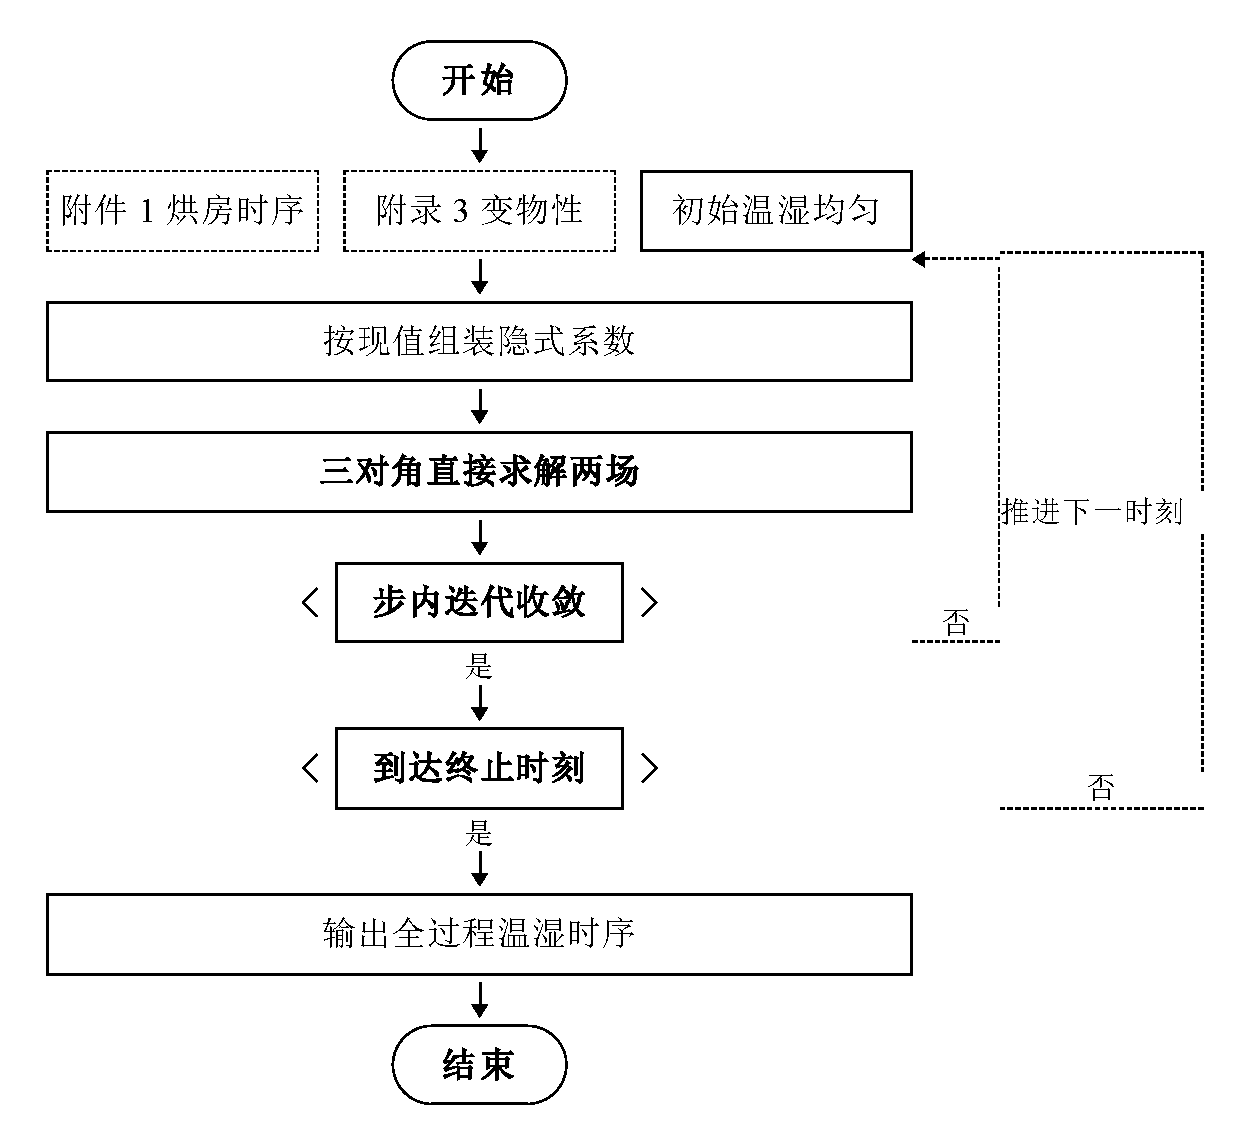
\includegraphics[width=0.86\textwidth,height=0.8\textheight,keepaspectratio]{../figures/fig_flow_q2.pdf}
  \caption{问题 2 全过程求解的双重迭代结构。主链是一次时间步内的动作；内侧回路
  为步内 Picard 非线性迭代，外侧回路为步间时间推进，两条回路都返回到系数组装，
  区别在于外侧回路先推进到下一时刻。虚线框表示题给数据。}
  \label{fig:flow-q2}
\end{figure}

两条回路的区别值得说清：内侧回路不推进时间，它反复在同一时刻上更新系数直至解不再变化，解决的是非线性；外侧回路推进时间，解决的是演化。两者都回到系数组装这一步，因为一旦解或时刻改变，物性和界面系数都必须重算。实算中恒温平台段每步只需三到五次内迭代即收敛，预热段因温度变化快，峰值为 12 次。

\subsection{扩散系数的双变量依赖}

扩散系数第一次同时依赖两个场，它是两个方程之间耦合的唯一通道，其形态决定了整个干燥过程的节奏，因此值得单独考察，见图~\ref{fig:diff-surface}。

\begin{figure}[htbp]
  \centering
  % 本图宽度取 0.93 而非横图默认的 0.90：该图 b 面板的刻度字号在原生画布上只有 8.0pt，
  % 按 0.90 插入后上页字号为 7.75pt，低于 8pt 可读下限；0.93 使其回到 8.01pt。
  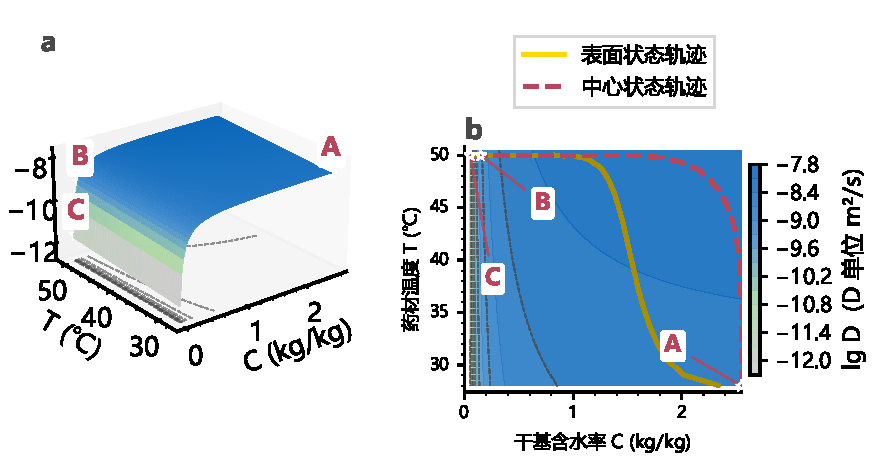
\includegraphics[width=0.93\textwidth,height=0.8\textheight,keepaspectratio]{../figures/fig_diff_surface.pdf}
  \caption{附录 3 扩散系数 $D(C,T)$ 的三维曲面与俯视投影。a：$\lg D$ 在
  $(C,T)$ 平面上的曲面，温度经 Arrhenius 因子起主导作用，含水率的修正相对
  次要；A、B、C 三点为全过程算例实际经过的状态，依次为初始态、含水率降至判据
  阈值时的状态与终态。b：同一函数的等高线俯视图，叠加中心与表面状态点的实算
  轨迹，可见两条轨迹沿温度方向先分离后合拢。}
  \label{fig:diff-surface}
\end{figure}

曲面沿温度方向的抬升幅度明显大于沿含水率方向，这说明升温对加快水分迁移的贡献超过变干对它的抑制，两者在干燥初期同时发生且方向相反。俯视图上中心与表面的两条轨迹在初期迅速分开，因为表面先升温也先变干；进入恒温段后两条轨迹又逐渐靠拢，因为温度趋于一致，差别只剩含水率。这一先分离后合拢的形态解释了为什么干燥速率在初期最快而后期显著放缓：初期是高温与高含水率叠加的有利区间，后期温度已无提升空间而含水率持续下降，扩散系数只能单向减小。

界面系数按式~\eqref{eq:iface} 的积分平均计算。以实算中一对相邻节点为例，两端含水率为 $2.55$ 与 $1.00$，端点扩散系数为 $1.3470\times10^{-8}$ 与 $1.0247\times10^{-8}$~m$^2$/s，积分平均给出 $1.2279\times10^{-8}$~m$^2$/s，严格落在两端点之间，与通量的物理含义一致。

\subsection{前三小时的温度与含水率}

按题目要求给出前三小时每半小时的结果，温度见表~\ref{tab:q2T}。完整分布按每秒、每 $0.1$~cm 输出，覆盖 $1$ 至 $10800$~s 共三小时，与本问所问的时间窗一致；全过程直到烘干结束的逐点分布由后一问以 $60$~s 间隔给出。

\begin{table}[H]
\centering
\caption{3 小时内药材的温度（单位：°C）}\label{tab:q2T}
\begin{tabular}{cccccc}
\toprule
\multirow{2}{*}{时间/h} & \multicolumn{5}{c}{到药材中心的距离/cm}\\
\cmidrule(lr){2-6}
 & 0 & 0.5 & 1 & 1.5 & 2 \\
\midrule
0.5 & 32.1893 & 32.3822 & 32.9660 & 33.9608 & 35.4132 \\
1.0 & 40.3812 & 40.5531 & 41.0601 & 41.8781 & 42.9977 \\
1.5 & 45.8460 & 45.9341 & 46.1923 & 46.6045 & 47.1397 \\
2.0 & 48.4497 & 48.4875 & 48.5980 & 48.7732 & 49.0031 \\
2.5 & 49.4667 & 49.4789 & 49.5134 & 49.5653 & 49.6609 \\
3.0 & 49.8494 & 49.8553 & 49.8745 & 49.9101 & 49.9664 \\
\bottomrule
\end{tabular}
\end{table}

表中五列在三小时末已收敛到同一个数值附近，径向温差不足 $0.12$~°C，温度场至此基本进入准稳态。同一批时刻与位置上的含水率结果列于表~\ref{tab:q2C}。

\begin{table}[H]
\centering
\caption{3 小时内药材的水分浓度（单位：kg/kg）}\label{tab:q2C}
\begin{tabular}{cccccc}
\toprule
\multirow{2}{*}{时间/h} & \multicolumn{5}{c}{到药材中心的距离/cm}\\
\cmidrule(lr){2-6}
 & 0 & 0.5 & 1 & 1.5 & 2 \\
\midrule
0.5 & 2.5499 & 2.5488 & 2.5254 & 2.3259 & 1.6486 \\
1.0 & 2.5255 & 2.4946 & 2.3578 & 2.0231 & 1.4710 \\
1.5 & 2.3859 & 2.3255 & 2.1344 & 1.8020 & 1.3475 \\
2.0 & 2.1708 & 2.1084 & 1.9236 & 1.6259 & 1.2310 \\
2.5 & 1.9566 & 1.9006 & 1.7360 & 1.4719 & 1.1166 \\
3.0 & 1.7662 & 1.7165 & 1.5702 & 1.3332 & 1.0081 \\
\bottomrule
\end{tabular}
\end{table}

两张表的对比清楚显示了两个场的分离。温度在两小时内就基本追上空气温度，第三小时末中心为 $49.8494$~°C、表面为 $49.9664$~°C，中心与表面之差已缩到 $0.12$~°C，整个截面进入准稳态；此后温度不再是限制因素。含水率则完全没有停下来的迹象，三小时末中心仍有 $1.7662$~kg/kg、表面为 $1.0081$~kg/kg，截面平均从 $2.5500$ 降到 $1.3824$~kg/kg，仅完成了到合格阈值所需降幅的一半左右。这一时间尺度的分离是全过程建模的核心事实：温度场很快退居背景，剩下的时间几乎全部花在水分向外扩散上。图~\ref{fig:q2-dual} 把两个场与物性的实时响应画在同一时间轴上。

\begin{figure}[htbp]
  \centering
  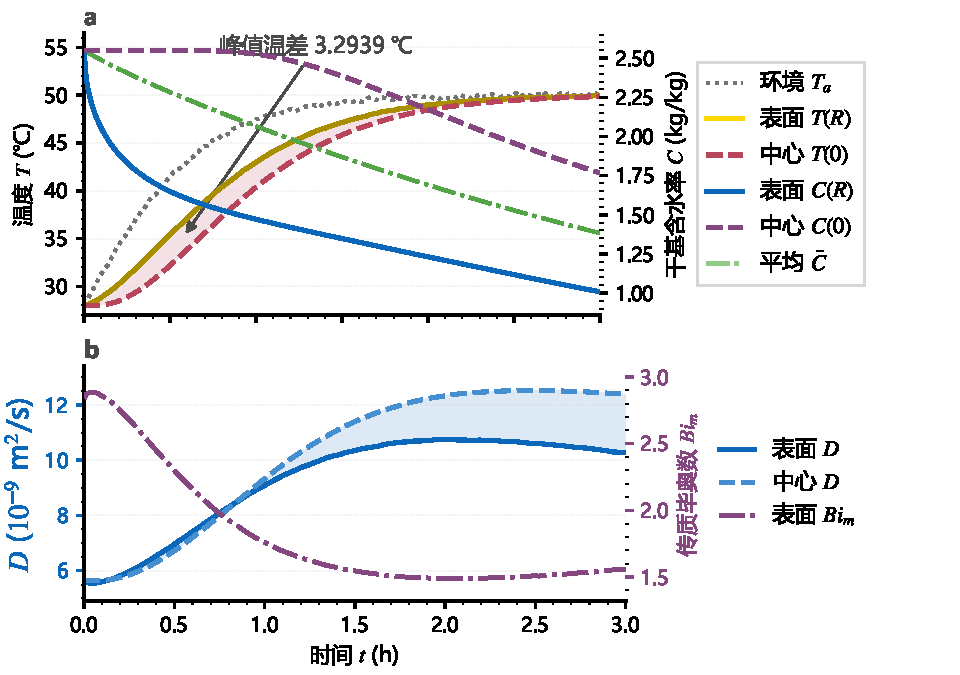
\includegraphics[width=0.9\textwidth,height=0.8\textheight,keepaspectratio]{../figures/fig_q2_dual.pdf}
  \caption{问题 2 前三小时的双轴演化与变物性响应。a：中心与表面温度追随空气
  温度上升，阴影为中心—表面温差带，同期三条含水率曲线同步下降；温度很快进入
  准稳态，含水率的下降贯穿整个过程，两者时间尺度相差一个量级以上。b：表面与
  中心扩散系数、表面传质毕奥数随含水率下降的实时变化，$D$ 在三小时内变化近
  一倍，故变物性不能用常数近似替代。}
  \label{fig:q2-dual}
\end{figure}

左图中温差阴影带在第一小时最宽而后迅速收窄，与表~\ref{tab:q2T} 中中心与表面之差从 $3.2$~°C 缩到 $0.12$~°C 相符；三条含水率曲线则保持大致平行地下行，未见收敛趋势。右图给出变物性不可用常数替代的直接证据：表面与中心的扩散系数在三小时内变化接近一倍，且两者之间始终存在可观差距；表面传质毕奥数同期持续增大，表明限制环节正在由表面对流向内部扩散转移。若把扩散系数冻结在任一时刻的取值，整个过程的速率都会被系统性地算错。

为了看清剖面形状随时间的变化，把六个时刻的径向剖面沿纵深方向排开，见图~\ref{fig:q2-ridgeline}。

\begin{figure}[htbp]
  \centering
  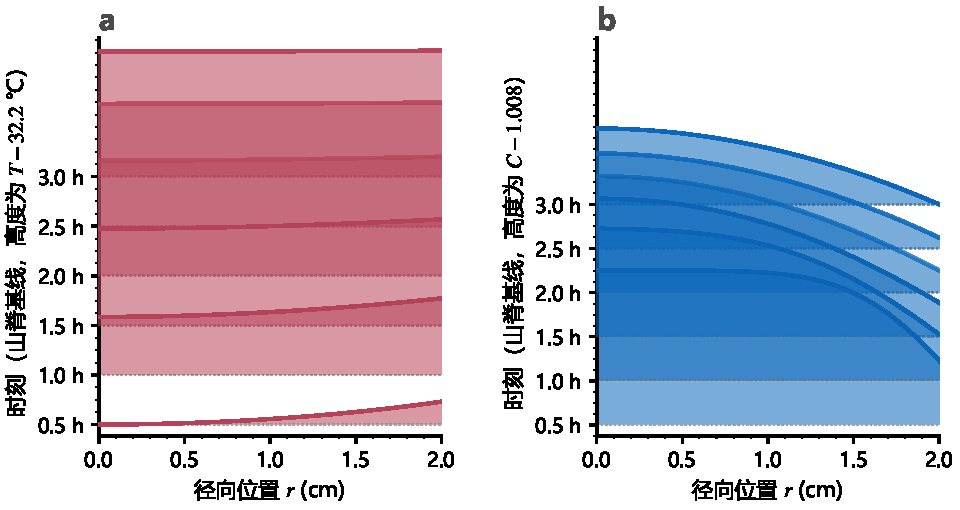
\includegraphics[width=0.9\textwidth,height=0.8\textheight,keepaspectratio]{../figures/fig_q2_ridgeline.pdf}
  \caption{问题 2 径向剖面的山脊图，6 个整时刻沿纵深方向排开（0.5\,h 间隔，
  21 个径向位置），纵向偏移即时间，每条山脊的高度是该时刻剖面相对全场最小值
  的抬升量。a：温度；b：含水率。干燥自表面向内推进，表面与轴线的落差先增大
  后随整体变干而趋缓，最湿位置始终在轴线附近。山脊排布用于避免六条剖面互相压线。}
  \label{fig:q2-ridgeline}
\end{figure}

温度一侧的山脊逐条变平，最后几条几乎成为水平线，对应温度场趋于均匀。含水率一侧的山脊则始终保持自轴线向表面下倾的形状，倾斜程度在第一小时后趋于稳定，说明干燥进入了一个形状大致自相似、整体逐步下移的阶段。所有时刻的最高点都落在轴线一侧，没有出现内部极值或局部反转，这一形态直接决定了下一问判据的取法：既然最湿的位置始终在轴线附近，要判断药材各处是否达标，就必须盯住径向最大值。本问的截面水分总量平衡残差为 $5.5\times10^{-13}$，与问题一同处机器精度量级。

\section{问题三：基于逐点判据的首次达标停时模型}

\subsection{合格判据的确定}

题目要求“药材各处的水分浓度应低于 0.15~kg/kg”。这句话在数学上有三种可能的落实方式，分别以表面含水率、截面平均含水率和全域最大含水率作为判据量，三者给出的时刻并不相同。表面最早达标，因为它直接与空气交换；截面平均次之，因为已经很干的外层能够把平均值拉下来，而轴线附近可能仍然偏湿；全域最大值最后达标，它成立时其余各点必然都已达标。既然题目要求的是“各处”，唯一与之对应的就是第三种。图~\ref{fig:criterion-logic} 把三者的关系整理成一次决策。

\begin{figure}[htbp]
  \centering
  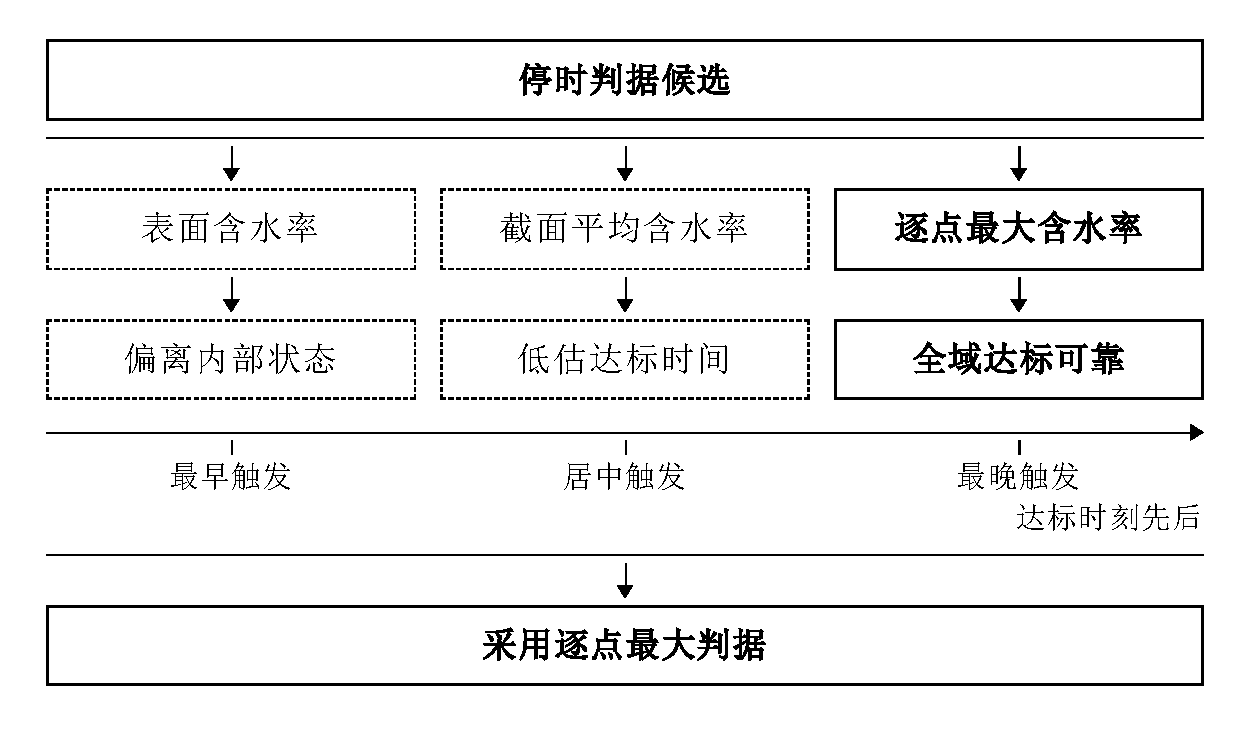
\includegraphics[width=0.9\textwidth,height=0.8\textheight,keepaspectratio]{../figures/fig_criterion_logic.pdf}
  \caption{停时判据的三候选决策。表面判据偏离内部状态，截面平均判据会低估达
  标时间，逐点最大判据能保证全域达标，故取后者；加粗框为采纳路径，虚线框为对照
  路径。底部时间轴只表示三种判据触发的先后次序，不含数值。}
  \label{fig:criterion-logic}
\end{figure}

图中底部时间轴上三个触发点的先后次序不依赖具体参数，它由三个判据量之间的不等关系直接决定。这一次序也说明误用前两种判据的后果是单向的：一定偏早，也就是把没有干透的药材判为合格。实算给出了这一偏差的量级，若改用截面平均含水率判据，达标时刻会提前 $21.70$~h，接近正确时长的四成。据此把烘干所需时间定义为

\begin{equation}
t_{\rm dry}=\inf\Big\{t>0:\ \max_{0\le r\le R_0}C(r,t)<C_{\rm th}\Big\},\qquad C_{\rm th}=0.15\ \mathrm{kg/kg}.
\label{eq:tdry}
\end{equation}

需要说明的是，判据写成径向最大值而不是中心值，是因为最湿位置的所在并非先验已知。本题在轴对称与外向失水的条件下，实算逐时刻核对确认 $\max_r C(r,t)$ 恒等于 $C(0,t)$，两者在 $10^{-12}$ 容差下完全一致，故最湿点始终在轴线；但判据的定义仍以最大值为准，这样在其他工况下也不会失效。

\subsection{停时的数值定位}

式~\eqref{eq:tdry} 是一个首次穿越时刻，它不能由某个显式表达式求出，只能在时间推进过程中逐步判断。求解流程如图~\ref{fig:flow-q3}。

\begin{figure}[htbp]
  \centering
  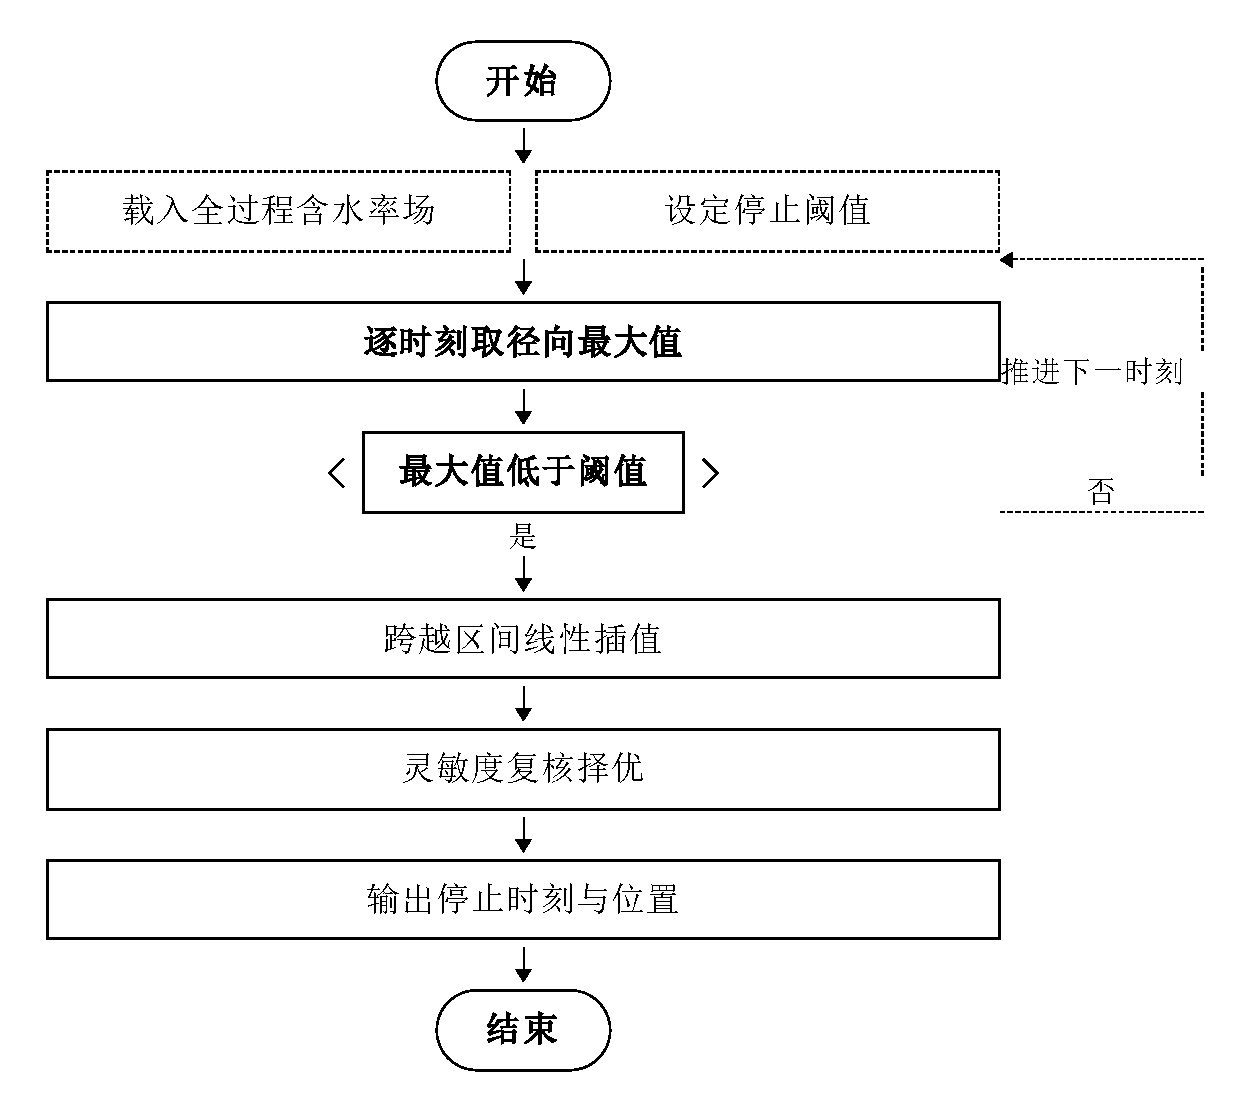
\includegraphics[width=0.86\textwidth,height=0.8\textheight,keepaspectratio]{../figures/fig_flow_q3.pdf}
  \caption{问题 3 停止时刻的判定流程。逐时刻取径向最大含水率与阈值比较，未达
  阈值则由右侧回路推进到下一时刻，已达阈值则在跨越区间内线性插值定位停时，再经
  灵敏度复核后输出。虚线框表示题给数据与外部给定的阈值。}
  \label{fig:flow-q3}
\end{figure}

流程的主体与问题二相同，新增的只是每步之后的一次比较和一次插值。由于输出间隔为 $60$~s，判据量恰好跨越阈值的那一刻一般落在两个输出时刻之间，需要在该区间内定位。设第 $k$ 个输出时刻的判据量仍高于阈值而第 $k+1$ 个已低于阈值，则按线性插值取

\begin{equation}
t_{\rm dry}=t_k+\frac{C_{\max}(t_k)-C_{\rm th}}{C_{\max}(t_k)-C_{\max}(t_{k+1})}\,\big(t_{k+1}-t_k\big).
\label{eq:interp}
\end{equation}

线性插值在此处足够可靠，因为判据量在阈值附近的下降速率极小且严格单调。实算的跨越区间为 $207060$ 至 $207120$~s，区间两端判据量分别为 $0.1500157$ 与 $0.1499982$，宽度恰为一个输出步，区间内不存在第二次穿越。

\subsection{烘干时长与全过程水分分布}

由式~\eqref{eq:interp} 定位得到

\begin{equation}
t_{\rm dry}=207113.776\ \mathrm{s}=57.5316\ \mathrm{h}=2.40\ \text{天}.
\label{eq:tdry3}
\end{equation}

该结果落在题目所述“烘干过程一般持续 2--3 天”的区间之内，为模型提供了一个来自题面本身的外部印证。达标时刻药材表面含水率已降至 $0.0526$~kg/kg，截面平均含水率为 $0.123903$~kg/kg，二者都远低于阈值，而轴线附近的含水率恰好抵达阈值。这一组数字正是“各处”与“平均”不能混用的直观说明：截面平均在轴线达标之前很久就已经跌破阈值。

按题目要求给出的水分浓度结果列于表~\ref{tab:q3C}。

\begin{table}[H]
\centering
\caption{药材烘干过程的水分浓度（单位：kg/kg）}\label{tab:q3C}
\begin{tabular}{cccccc}
\toprule
\multirow{2}{*}{时间/h} & \multicolumn{5}{c}{到药材中心的距离/cm}\\
\cmidrule(lr){2-6}
 & 0 & 0.5 & 1 & 1.5 & 2 \\
\midrule
6  & 1.0176 & 0.9888 & 0.9021 & 0.7555 & 0.5332 \\
12 & 0.4569 & 0.4439 & 0.4037 & 0.3303 & 0.1647 \\
18 & 0.2992 & 0.2919 & 0.2691 & 0.2256 & 0.0847 \\
24 & 0.2380 & 0.2330 & 0.2169 & 0.1857 & 0.0665 \\
30 & 0.2060 & 0.2020 & 0.1893 & 0.1642 & 0.0598 \\
36 & 0.1860 & 0.1826 & 0.1719 & 0.1505 & 0.0566 \\
42 & 0.1722 & 0.1692 & 0.1598 & 0.1408 & 0.0548 \\
48 & 0.1619 & 0.1593 & 0.1508 & 0.1335 & 0.0537 \\
54 & 0.1539 & 0.1515 & 0.1437 & 0.1278 & 0.0530 \\
烘干结束时间 & 0.1500 & 0.1477 & 0.1402 & 0.1249 & 0.0526 \\
\bottomrule
\end{tabular}

\vspace{0.6em}
\begin{minipage}{0.92\textwidth}
\footnotesize 末行为式~\eqref{eq:tdry3} 给出的烘干结束时间 $t_{\rm dry}=57.5316$~h。按式~\eqref{eq:tdry}
的定义，$t_{\rm dry}$ 正是判据量抵达阈值的时刻，故该行轴线处的数值等于阈值 $0.1500$；
严格低于阈值在其后的任意时刻成立，例如下一个输出时刻（晚 $6.2$~s）轴线含水率为
$0.1499982$~kg/kg。
\end{minipage}
\end{table}

% 同上：行内数学密集的中文段落，补一点应急伸展量。
{\emergencystretch=2.5em
表中数据呈现出显著的前快后慢：前 $12$~h 轴线含水率由 $2.5500$ 一路降到 $0.4569$~kg/kg，去掉了总降幅的八成以上；而从 $0.4569$ 降到阈值却用掉了剩下的 $45$~h。造成这一转折的正是扩散系数随变干而急剧减小。同时可以看到，表面在 $12$~h 时已降到 $0.1647$、$18$~h 时降到 $0.0847$~kg/kg，此后基本不再变化，而轴线仍在缓慢下降，整个后半程的进展几乎全部发生在药材内部。图~\ref{fig:q3-criterion} 给出三个判据量的完整下降过程与停时邻域的放大。\par}

\begin{figure}[htbp]
  \centering
  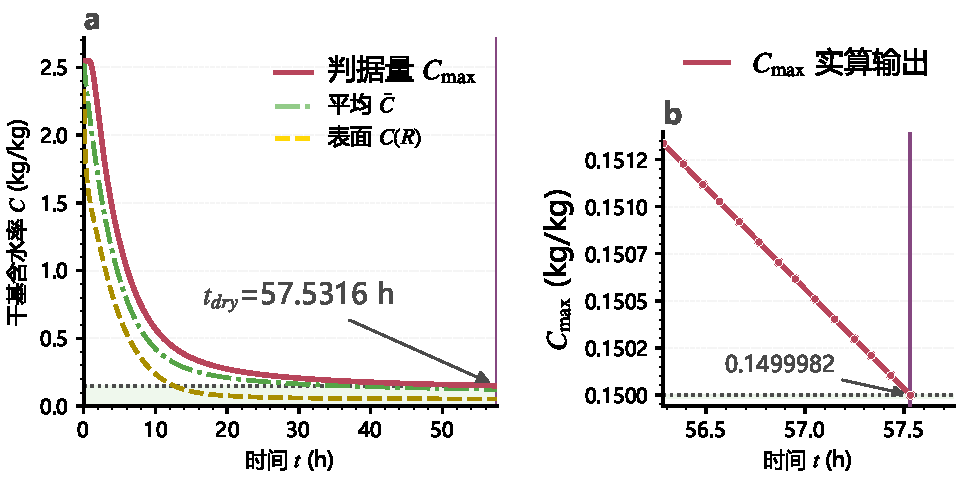
\includegraphics[width=0.9\textwidth,height=0.8\textheight,keepaspectratio]{../figures/fig_q3_criterion.pdf}
  \caption{问题 3 停时判据的实算依据。a：判据量 $\max_r C$、表面含水率与截面
  平均含水率三条曲线的全程下降，水平点线为阈值 0.15，绿色底带为达标区；三条
  曲线的先后次序印证了平均判据偏早、表面判据更偏早。b：停时前 1.25\,h 的邻域
  放大（1\,min 分辨率的实算输出点），显示判据被单调穿越且只穿越一次，故插值
  定位的停时唯一。轴对称条件下最湿位置恒在轴线，$\max_r C$ 即中心值。}
  \label{fig:q3-criterion}
\end{figure}

左图中三条曲线自上而下依次是判据量、截面平均和表面含水率，它们与阈值线的交点从右到左排列，与图~\ref{fig:criterion-logic} 所给的次序一致，且交点之间的水平距离相当可观，说明判据取法的影响不是可以忽略的细节。右图把停时前 $1.25$~h 放大后可以看到，实算输出点排成一条平缓且严格单调的直线，穿越阈值时既无震荡也无二次穿越，式~\eqref{eq:interp} 的线性插值在这样的局部形态下几乎没有额外误差。

最后把一维径向解按轴对称铺回圆截面，得到四个时刻的水分分布快照，见图~\ref{fig:q3-frames}。

\begin{figure}[htbp]
  \centering
  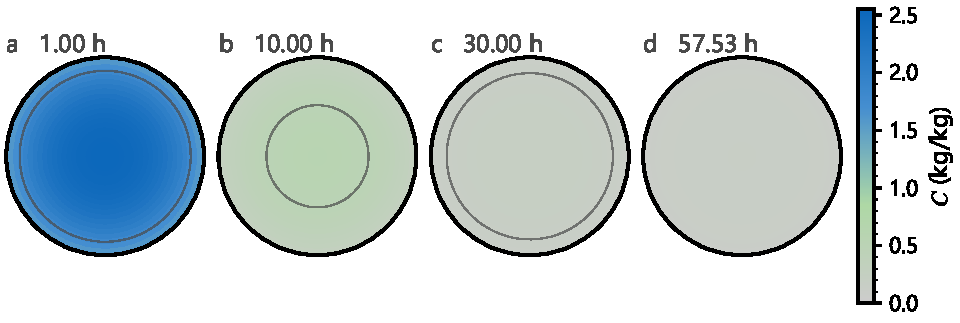
\includegraphics[width=0.9\textwidth,height=0.8\textheight,keepaspectratio]{../figures/fig_q3_frames.pdf}
  \caption{问题 3 圆截面水分场的四帧俯视快照（1、10、30\,h 与停时），把一维
  径向解按轴对称铺成圆盘。四帧共用同一色标以便跨帧比较，细等值线为 0.15、
  0.5、1.0、1.8 四级。干燥前沿由外向内推进，末帧整盘进入达标色域，直观说明
  全域达标是在最湿的轴线越过阈值那一刻实现的。}
  \label{fig:q3-frames}
\end{figure}

四帧连起来看，$1$~h 时只有薄薄一圈外缘变干，$10$~h 时干燥前沿已推进到半径中段，$30$~h 时整盘颜色接近均匀但轴心仍有一小块未达标，到停时那一帧才整盘进入达标色域。最后一帧中轴心残留的浅色斑点面积很小，却决定了整炉药材的出炉时刻，这正是逐点判据在工程上的意义所在。本问的截面水分总量平衡残差为 $5.5\times10^{-13}$，全程共 $3452$ 个输出时刻、每时刻 $21$ 个径向位置的完整水分场随结果文件一并给出。

\section{问题四：收缩域上的移动边界模型}

\subsection{实测半径与物质坐标变换}

本问的求解区域不再固定。附件 2 给出 $145$ 个时刻的药材半径，覆盖 $0$ 至 $259200$~s，半径由 $2.000$~cm 单调减到序列末端的 $1.198$~cm，自 $126000$~s 起即稳定在 $1.200$~cm 附近，序列末端的收缩比为 $0.599$，截面积只剩初始的 $0.3588$；后文用到的停时处收缩比按该时刻的半径另行取值。半径序列的形态见图~\ref{fig:radius-shrink}。

\begin{figure}[htbp]
  \centering
  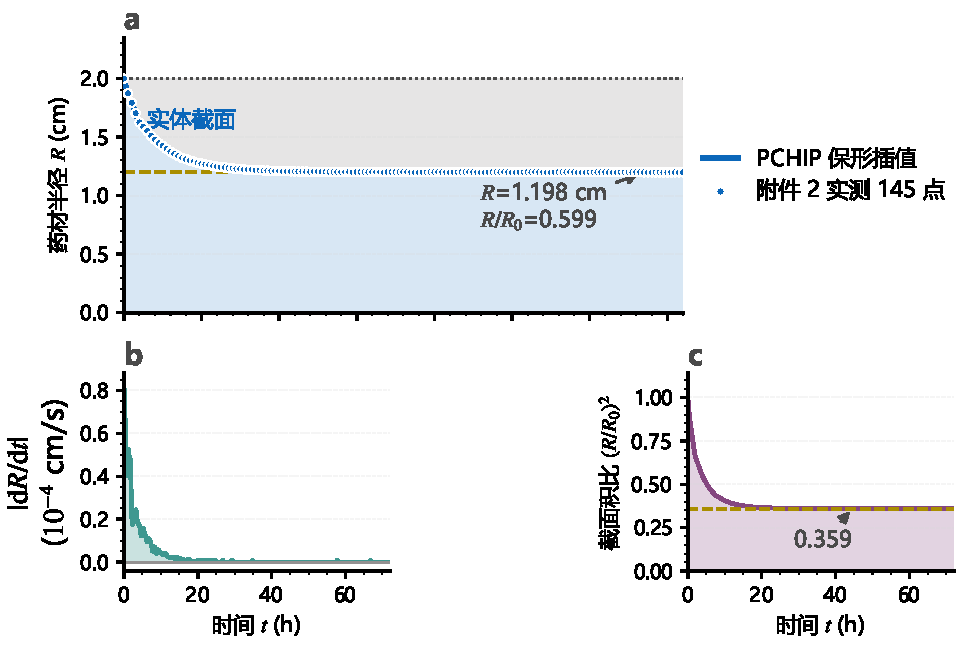
\includegraphics[width=0.9\textwidth,height=0.8\textheight,keepaspectratio]{../figures/fig_radius_shrink.pdf}
  \caption{附件 2 实测的药材半径收缩过程。a：散点为 145 点实测值，曲线为
  PCHIP 保形插值（保形以避免插值曲线出现非物理的半径回弹），深色填充为药材
  实体截面，浅色为已收缩掉的区域；b：收缩速率 $|\mathrm{d}R/\mathrm{d}t|$；
  c：截面积比 $(R/R_0)^2$。终值半径与收缩比直接进入问题 4 的物质坐标变换。}
  \label{fig:radius-shrink}
\end{figure}

收缩集中在前二十小时，此后速率趋于零，这与含水率的前快后慢是一致的：失水停止，收缩自然也停止。热风干燥的实测研究也报告了同一现象，即收缩量与失水量在整个过程中同步演化，且两者共同改变有效扩散系数\upcite{ning2025shrinkage}。插值方式的选择在此处有实际后果。三次样条会在拐点附近产生过冲，使插值曲线出现半径回升这种非物理的结果；分段三次 Hermite 保形插值则保持原始数据的单调性，导数由插值函数解析求出而非对原始数据作差分，避免出现半小时周期的阶梯脉冲。

区域随时间变形，固定域上的离散格式不能直接套用。本文引入以当前半径归一的物质坐标

\begin{equation}
s=\frac{r}{R(t)}\in[0,1],
\label{eq:mapping}
\end{equation}

在径向仿射收缩下，同一个 $s$ 始终标记同一份干物质，因此 $s$ 是物质标签而非固定于实验室的空间坐标。链式法则给出

\begin{equation}
\left.\frac{\partial C}{\partial t}\right|_{r}
=\left.\frac{\partial C}{\partial t}\right|_{s}
-\frac{s\dot R}{R}\frac{\partial C}{\partial s},
\qquad
\frac{\partial}{\partial r}=\frac{1}{R(t)}\frac{\partial}{\partial s} .
\label{eq:chain}
\end{equation}

把式~\eqref{eq:chain} 代回式~\eqref{eq:mass}，表观对流项与坐标变换产生的项精确相消，剩下纯扩散形式

\begin{equation}
\left.\frac{\partial C}{\partial t}\right|_{s}
=\frac{1}{R^2(t)}\cdot\frac{1}{s}\frac{\partial}{\partial s}
\!\left(s\,D(C,T)\frac{\partial C}{\partial s}\right),
\qquad 0<s<1,
\label{eq:q4c}
\end{equation}

\begin{equation}
\left.\frac{\partial C}{\partial s}\right|_{s=0}=0,
\qquad
\left.-\frac{D(C,T)}{R(t)}\frac{\partial C}{\partial s}\right|_{s=1}
=h_m\big[C(1,t)-C_a(t)\big].
\label{eq:q4bc}
\end{equation}

温度方程同构，只需把 $D$ 换成 $\lambda$、右端整体除以 $\rho c_p$、边界系数换成 $h$ 与 $T_a$。方程中不再出现半径变化率，但收缩并未被忽略：$R(t)$ 出现在式~\eqref{eq:q4c} 的 $1/R^2(t)$、式~\eqref{eq:q4bc} 的 $1/R(t)$ 以及控制体的物理体积 $R^2(t)V_i$ 三处，每一处都随时间变化。这一变换的几何含义可由图~\ref{fig:mech-moving} 看出。

\begin{figure}[htbp]
  \centering
  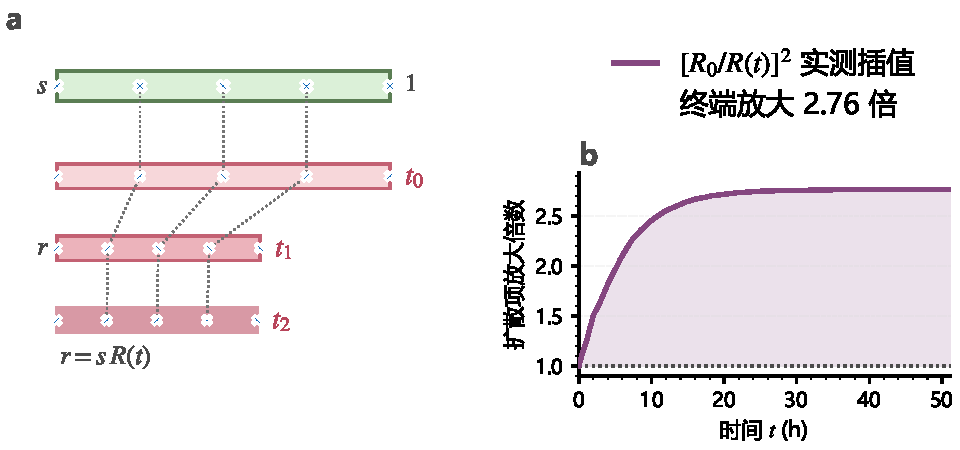
\includegraphics[width=0.9\textwidth,height=0.8\textheight,keepaspectratio]{../figures/fig_mech_moving.pdf}
  \caption{物质坐标映射与收缩放大。a：固定域上的节点随物质一起向轴线移动，
  表面恒落在 $s=1$；点线为同一物质点在三个时刻的轨迹。b：扩散项前
  $1/R^2(t)$ 的放大倍数随时间的变化，由附件 2 实测半径算出。}
  \label{fig:mech-moving}
\end{figure}

左图中三条点线是同一物质点在三个时刻的位置，它们都在向轴线靠拢，而其 $s$ 坐标不变，这正是“网格随物质移动”的含义；表面始终落在 $s=1$，边界条件的施加位置因此不随时间改变。右图给出收缩加速干燥的主要定量来源：半径由 $2$~cm 减到 $1.2$~cm 时，$1/R^2$ 增大 $2.78$ 倍，同样的含水率落差被压缩在更短的物理距离上，梯度随之增大；式~\eqref{eq:q4bc} 的 $1/R(t)$ 与控制体体积的变化同向叠加，量级小于此项。

物质坐标与实验室坐标是同一个方程的两种写法，数学上等价，本文选择前者是因为它把边界固定在坐标端点、且不需要用到半径的导数。作为独立对照，本文也按实验室坐标的写法实现了一支算例，用于交叉检验实现的正确性，两条路线的关系见图~\ref{fig:flow-q4}。

\begin{figure}[htbp]
  \centering
  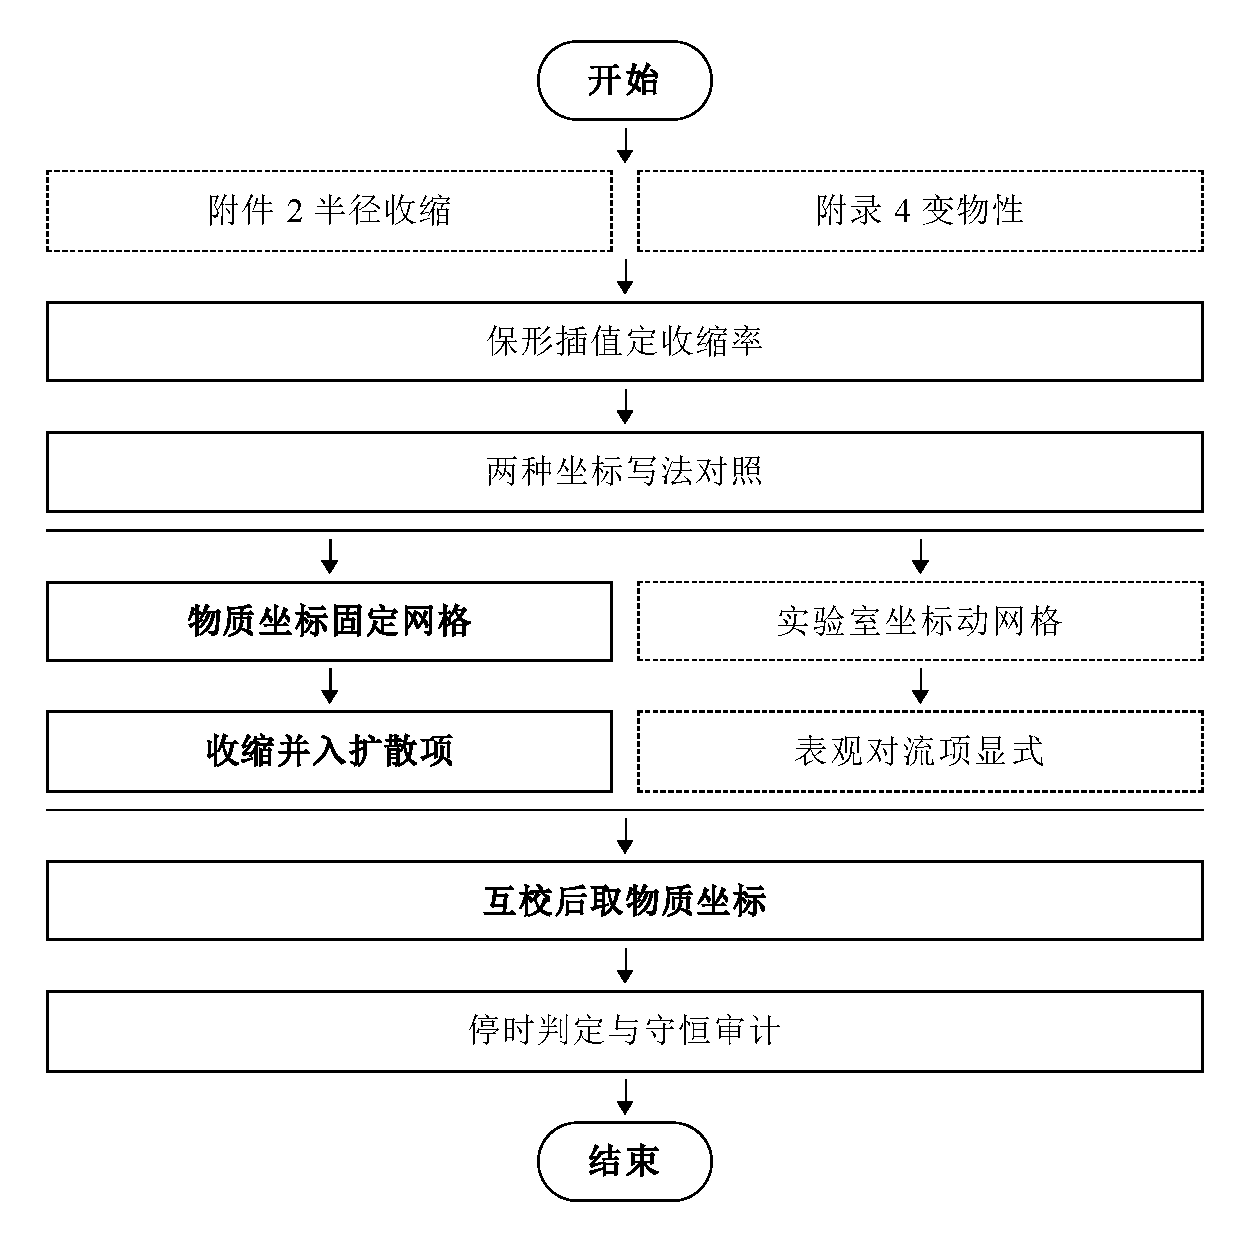
\includegraphics[width=0.8\textwidth,height=0.8\textheight,keepaspectratio]{../figures/fig_flow_q4.pdf}
  \caption{问题 4 收缩域的两条坐标路线。共同输入后分为物质坐标固定网格与实
  验室坐标动网格两支，收缩效应分别并入扩散项与显式表观对流项；加粗框为采纳的
  物质坐标支，虚线框为实验室坐标对照支，两支互校后取前者为主模型，再做停时判定
  与干物质守恒校核。}
  \label{fig:flow-q4}
\end{figure}

两支共用输入、物性、判据与求解器，仅在收缩效应的写法上分开。互校的判别标准取干物质守恒：单位长度的干物质总量在整个过程中不应改变。两支的残差与互校结果在第~\ref{sec:q34} 小节一并讨论。

\subsection{烘干时长与收缩域内的水分分布}

本问物性改用附录 4，即式~\eqref{eq:app4}，判据仍为式~\eqref{eq:tdry}、定位仍按式~\eqref{eq:interp}。所得烘干时长为

\begin{equation}
t_{\rm dry}=184098.165\ \mathrm{s}=51.1384\ \mathrm{h}=2.13\ \text{天},
\label{eq:tdry4}
\end{equation}

比问题三的 $57.5316$~h 提前 $6.3932$~h，相对减少 $11.11\%$，同样落在题目所述两到三天的区间内。该时刻半径为 $1.2000$~cm，收缩比恰为 $0.6000$；停时对应的时间 $1.84\times10^5$~s 落在附件 2 覆盖的 $72$~h 之内，无需对半径序列作任何外推。达标时刻表面含水率为 $0.0526$~kg/kg，截面平均含水率为 $0.118200$~kg/kg。

按题目要求给出的水分浓度结果列于表~\ref{tab:q4C}。

\begin{table}[H]
\centering
\caption{收缩情形下药材烘干过程的水分浓度（单位：kg/kg）}\label{tab:q4C}
\begin{tabular}{ccccccc}
\toprule
\multirow{2}{*}{时间/h} & \multicolumn{5}{c}{到药材中心的距离/cm} & \multirow{2}{*}{药材表面}\\
\cmidrule(lr){2-6}
 & 0 & 0.5 & 1 & 1.5 & 2 & \\
\midrule
6  & 1.7189 & 1.5366 & 1.0217 & --- & --- & 0.4205 \\
12 & 0.7383 & 0.6551 & 0.4086 & --- & --- & 0.1671 \\
18 & 0.4093 & 0.3690 & 0.2396 & --- & --- & 0.0893 \\
24 & 0.2854 & 0.2613 & 0.1788 & --- & --- & 0.0674 \\
30 & 0.2265 & 0.2095 & 0.1491 & --- & --- & 0.0595 \\
36 & 0.1930 & 0.1797 & 0.1315 & --- & --- & 0.0560 \\
42 & 0.1714 & 0.1604 & 0.1199 & --- & --- & 0.0541 \\
48 & 0.1562 & 0.1469 & 0.1115 & --- & --- & 0.0530 \\
烘干结束时间 & 0.1500 & 0.1412 & 0.1079 & --- & --- & 0.0526 \\
\bottomrule
\end{tabular}

\vspace{0.6em}
\begin{minipage}{0.96\textwidth}
\footnotesize 破折号表示该径向位置在对应时刻已落在药材之外：$6$~h 时半径已小于 $1.5$~cm，
故 $1.5$~cm 与 $2$~cm 两列此后不再有药材存在，按题意留空而不填零，以免与“已经很干”混淆。
末列“药材表面”跟随移动边界 $R(t)$ 取值。末行为式~\eqref{eq:tdry4} 给出的烘干结束时间
$t_{\rm dry}=51.1384$~h；与表~\ref{tab:q3C} 同理，该时刻判据量恰等于阈值 $0.1500$，
严格低于阈值在其后成立，下一个输出时刻（晚 $41.8$~s）轴线含水率为 $0.149979$~kg/kg。
\end{minipage}
\end{table}

与表~\ref{tab:q3C} 逐行对照可以看到，收缩情形下前 $6$~h 的轴线含水率还高于固定域（$1.7189$ 对 $1.0176$），说明附录 4 的扩散系数确实更小、初期干燥更慢；此后两者的差距逐步缩小，轴线含水率之比由 $6$~h 的 $1.69$ 降到 $24$~h 的 $1.20$、$36$~h 的 $1.04$，在 $36$ 至 $42$~h 之间才转为收缩情形更低（$42$~h 为 $0.99$，$48$~h 为 $0.97$），最终使总时长更短。这种先慢后快的交叉说明净时长的符号不能凭定性推理断定。收缩域内水分场的完整图景见图~\ref{fig:q4-contour}。

\begin{figure}[htbp]
  \centering
  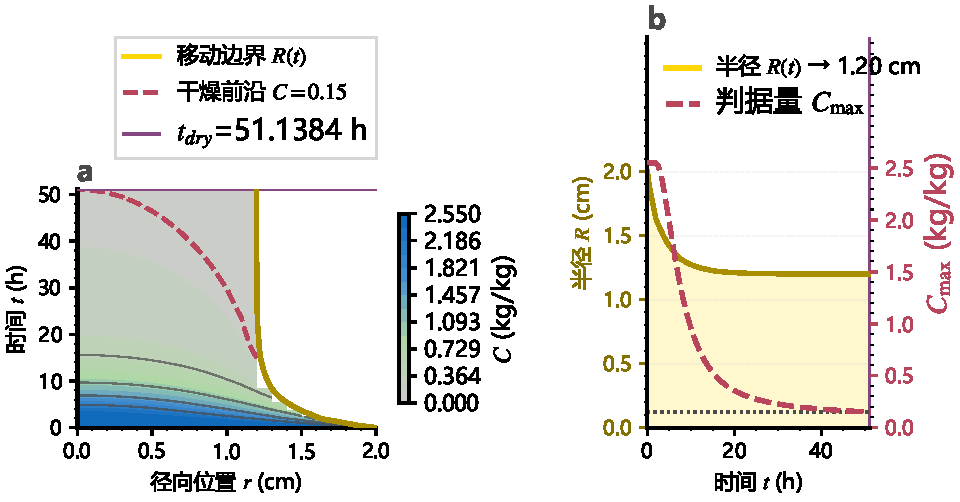
\includegraphics[width=0.9\textwidth,height=0.8\textheight,keepaspectratio]{../figures/fig_q4_contour.pdf}
  \caption{问题 4 收缩域内的水分场。a：$(r,t)$ 平面上的含水率等高线，实心区为
  药材本体，移动边界 $R(t)$ 右侧留白即已收缩掉的区域（不填零值以免与“很干”
  混淆）；粗虚线为干燥前沿 $C=0.15$，它与 $R(t)$ 的交汇决定停时。b：半径
  $R(t)$ 与判据量 $C_{\max}$ 的同步演化，竖线为停时；判据量在半径已趋平后
  才穿越阈值，说明停时由水分扩散而非几何收缩直接决定。}
  \label{fig:q4-contour}
\end{figure}

左图的留白区域是本图与图~\ref{fig:q3-frames} 最直观的差别：随着时间推移，药材本体在图上不断变窄，等值线被挤压向左，密集程度明显高于固定域的情形。右图的两条曲线揭示了一个容易误判的因果关系：半径在约 $35$~h 后已基本不再变化，而判据量还要再经过十余小时才穿越阈值，因此停时直接由水分扩散的进度决定，收缩的作用是在此之前就已经通过压缩扩散路径“预支”掉的。

\subsection{两个效应的分解与守恒校核}\label{sec:q34}

问题四与问题三的差别同时来自物性组的更换与几何的收缩。为把两者分开，本文在同一求解器、同一网格与同一判据下追加一个只换物性而保持半径不变的隔离算例，结果列于表~\ref{tab:q34}。

\begin{table}[H]
\centering
\caption{问题三到问题四的效应分解}\label{tab:q34}
\begin{tabular}{lcc}
\toprule
算例 & $t_{\rm dry}$/h & 相对上一行 \\
\midrule
问题三：附录 3 物性，固定半径 & 57.5316 & 基准 \\
只换附录 4 物性，半径仍固定 & 129.9252 & $+125.8\%$ \\
附录 4 物性并计入实测半径收缩 & 51.1384 & $-60.6\%$ \\
\bottomrule
\end{tabular}
\end{table}

两个效应的方向相反而量级都很大。附录 4 的扩散系数前因子比附录 3 小近一个数量级，虽然浓度项的指数更平缓（$-0.30/C$ 对 $-0.45/C$）能部分补偿，净效应仍使干燥慢一倍以上；几何收缩则通过 $1/R^2$ 把干燥加快约六成。表中两个百分数各以上一行为基准，因而是相继作用而非可以相加：$57.5316$~h 先被物性拉长到 $129.9252$~h，再被收缩压回 $51.1384$~h，最终相对问题三只提前 $11.1\%$。若只凭“收缩使干燥更快”就断言问题四明显快于问题三，或只凭“附录 4 扩散更弱”就断言更慢，都会得到错误结论。这一分解与守恒校核并列于图~\ref{fig:q34-compare}。

\begin{figure}[htbp]
  \centering
  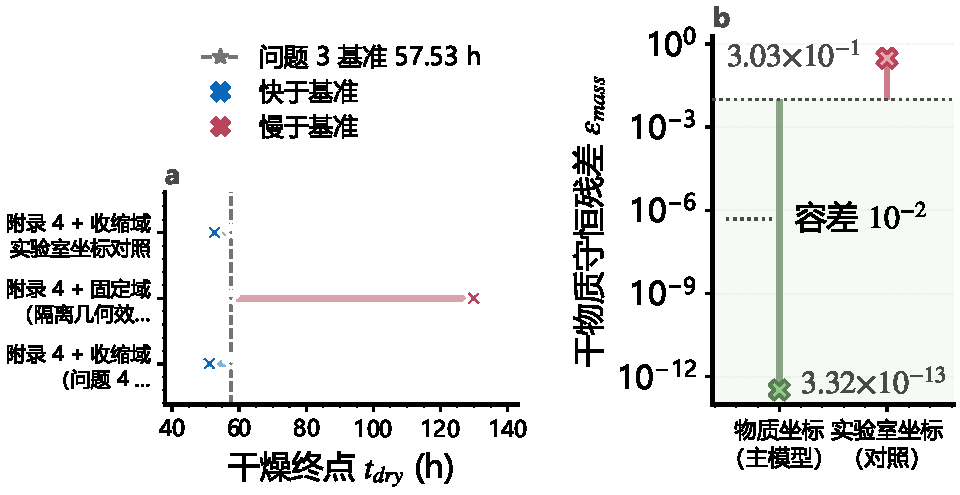
\includegraphics[width=0.9\textwidth,height=0.8\textheight,keepaspectratio]{../figures/fig_q34_compare.pdf}
  \caption{问题 3 与问题 4 的效应分解与实现校核。a：哑铃图，每行一个分支，
  左端固定为问题 3 的基准停时，右端为该分支实算值，连线长度即该处理的净效应；
  可见单换附录 4 物性（固定域）使干燥显著变慢，再叠加半径收缩才把停时拉回并
  超过基准，两个效应方向相反。b：两支实现的干物质守恒残差，以 $10^{-2}$
  容差线为基线的杆状图（对数纵轴上柱长会随人为地板而变，故不用柱状）；物质
  坐标残差处于舍入量级，实验室坐标一支达 30\%，据此定位到该支把已被坐标变换
  吸收的边界运动又显式计入了一次。}
  \label{fig:q34-compare}
\end{figure}

左图把表~\ref{tab:q34} 画成哑铃形式，两条连线一长一短、方向相反，长度差即最终的净效应。右图是干物质守恒的校核结果，它的作用超出了常规校验。物质坐标一支的残差为 $3.3\times10^{-13}$，处于浮点舍入累积的量级；实验室坐标一支却达到 $30.3\%$，远超 $1\%$ 的容差。既然两种写法在数学上等价，这样悬殊的差别只能来自实现本身。据此复查发现，该支在保留表观对流项的同时，扩散项仍按物质坐标的形式带有 $1/R^2$ 因子，等于把边界运动计入了两次，其停时因而系统性偏慢 $2.93\%$（$52.6377$~h）。这里记录这一诊断，是因为它说明守恒校核能捕捉到单纯比较停时数值无法发现的实现错误，而不是说明某一种坐标写法本身更优。

收缩方式本身也可以由守恒关系独立判定。单位长度的干物质总量守恒给出

\begin{equation}
\rho_{\rm d}(t)\,R^2(t)=\rho_{\rm d}(0)\,R^2(0),\qquad
\rho_{\rm d}=\frac{\rho(C)}{1+C},
\label{eq:drymass}
\end{equation}

由附录 4 的密度公式与初始含水率得 $\rho_{\rm d}(0)=278.73$~kg/m$^3$。把停时处的收缩比 $R(t_{\rm dry})/R_0=0.6000$ 代入式~\eqref{eq:drymass}，若按径向仿射收缩反推，干物质密度为 $774.26$~kg/m$^3$；若改按各向同性收缩反推，则为 $1290.43$~kg/m$^3$。这两个数值需要与附录 4 密度公式的两个自然参照相比：其一是含水率趋零时的绝干截距 $760$~kg/m$^3$，径向收缩偏高 $1.9\%$，各向同性收缩偏高 $69.8\%$；其二是按终态平均含水率算得的 $\rho(\bar C)/(1+\bar C)=689.18$~kg/m$^3$，径向收缩偏高 $12.35\%$，各向同性收缩偏高 $87.24\%$。两个参照下的结论一致：径向仿射收缩与题给数据相容到十几个百分点以内，各向同性收缩则偏离近一倍，据此排除后者。这一判断使用的是附件 2 的几何序列与附录 4 的密度公式两项互不相干的题给信息，因而构成对假设（6）的独立支持。

\section{数值可信性的多重校验}

前四问的结论全部来自同一套离散实现，因此有必要说明这些数字在多大程度上独立于离散参数与实现细节。本章给出四组证据：离散参数的收敛性、与解析解的对照、离散守恒的恒等性，以及一组答案可以先验判定的退化算例。四者的价值在于失效原因互不重叠：收敛性只能说明解对网格与时间步不敏感，却无法排除方程被写错；解析解能查出方程写错，却只在常物性下可用；守恒残差对通量组装的错误极其灵敏，但对系数取值的错误不敏感；退化算例则直接检验极限行为是否正确。

\subsection{离散参数的收敛性与解析解对照}

空间收敛以三个问题各自最敏感的输出量为指标：问题一取表面含水率，因为它位于边界层内、对径向分辨最挑剔；问题三与问题四取停时，因为它是本文的主要交付量。网格由 $N=20$ 加倍到 $40$ 时，三者依次变化 $0.1069\%$、$0.0521\%$、$0.0547\%$，第一项已超出 $0.1\%$ 的容差；再由 $40$ 加倍到 $80$ 时，三者降为 $0.0262\%$、$0.0137\%$、$0.0140\%$，全部远在容差之内。生产网格因此取 $N=40$：更粗一档不能通过检验，更细一档不改变任何一位有效数字。

时间收敛在固定网格上考察。以问题一的中心温度为指标，时间步自 $2$~s 起逐次减半至 $0.25$~s，另在减半序列之外加算一档更细的 $0.1$~s。减半序列内相邻两档之差依次为 $1.202\times10^{-3}$、$6.006\times10^{-4}$、$3.002\times10^{-4}$~°C，每档约为前一档的一半，据此按

\begin{equation}
p=\log_2\frac{y(\Delta t)-y(\Delta t/2)}{y(\Delta t/2)-y(\Delta t/4)},
\qquad
y^{\ast}=y(\Delta t/2)+\frac{y(\Delta t/2)-y(\Delta t)}{2^{p}-1}
\label{eq:order}
\end{equation}

由 $\Delta t=1$、$0.5$、$0.25$~s 这三档算出观测阶为 $1.0005$，与后向 Euler 的理论一阶完全一致；$y$ 对 $\Delta t$ 的线性拟合决定系数为 $0.9999999$，说明高阶残项在该区间内可以忽略。式~\eqref{eq:order} 给出的 Richardson 外推极限为 $33.5752$~°C，与同一支最细的 $\Delta t=0.1$~s 一档相差 $1.2\times10^{-4}$~°C，相对量级为 $10^{-6}$；表~\ref{tab:q1T} 所报的 $33.5753$~°C 与该极限只差末位一个单位。问题三的时间步安排另行考察：恒温平台段由 $120$~s 减半到 $60$~s 使停时变化 $0.0811\%$，生产取值 $60$~s 相对最细的 $10$~s 偏差 $0.0677\%$。网格加倍与时间步减半同时进行时，问题一变化 $0.0291\%$、问题三变化 $0.0544\%$，两项误差没有相互放大。

解析解对照需要一个有闭式答案的算例，因此另设一支：物性取常值、空气温度冻结在实测平台值 $49.9989$~°C，此时热方程退化为常系数线性问题，圆柱在第三类边界下的经典级数解为

\begin{equation}
\frac{T(r,t)-T_a}{T_0-T_a}
=\sum_{n=1}^{\infty}\frac{2\,{\rm Bi}_h}{(\zeta_n^{2}+{\rm Bi}_h^{2})J_0(\zeta_n)}
\,J_0\!\left(\frac{\zeta_n r}{R_0}\right)
\exp\!\left(-\frac{\zeta_n^{2}\alpha t}{R_0^{2}}\right),
\label{eq:bessel}
\end{equation}

式~\eqref{eq:bessel} 中特征值 $\zeta_n$ 取 $\zeta J_1(\zeta)={\rm Bi}_h J_0(\zeta)$ 的正根，前三个为 $1.4185$、$4.1665$、$7.2085$。取十项求和，$1800$~s 时中心温度的解析值为 $43.9623$~°C、表面为 $46.6376$~°C。需要说明的是这一数值与表~\ref{tab:q1T} 的 $33.5753$~°C 并不矛盾：后者的空气温度按附件 1 实测逐时刻变化、半小时内尚在升温途中，而此处为构造闭式解把空气温度整段固定在平台值，两者是不同的算例。数值解在 $N=80$ 上把时间步由 $1$~s 减到 $0.05$~s，中心温度与解析值的绝对偏差由 $3.94\times10^{-3}$~°C 单调降到 $2.20\times10^{-4}$~°C，相邻档之间的观测阶为 $0.99$、$0.97$、$0.92$。三组证据画在图~\ref{fig:verification} 中。

\begin{figure}[htbp]
  \centering
  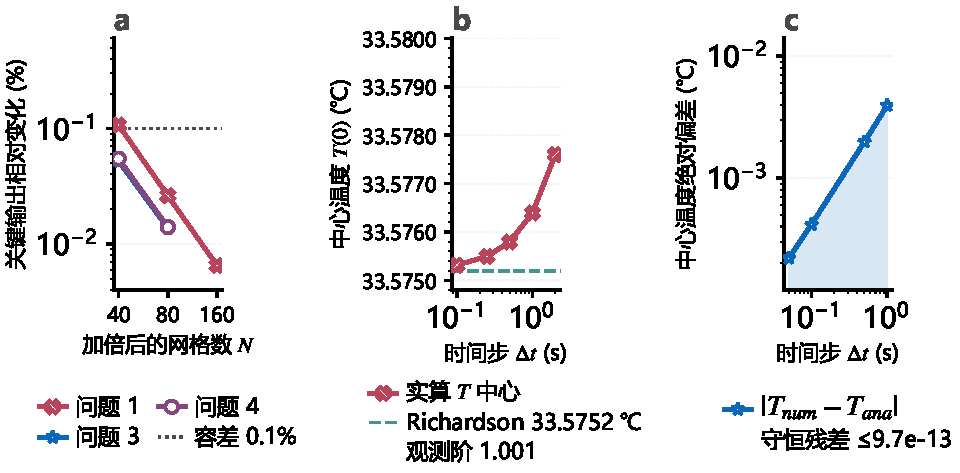
\includegraphics[width=0.9\textwidth,height=0.8\textheight,keepaspectratio]{../figures/fig_verification.pdf}
  \caption{数值可信性三联校验。a：三个问题的关键输出随网格逐次加倍的相对变化，
  仅问题一最粗的一档在 0.1\% 容差线之上，生产网格 $N=40$ 及其后各档均落在线下；
  b：固定网格下中心温度随时间步收敛，观测阶约为 1，
  与后向 Euler 的理论一阶一致，虚线为 Richardson 外推极限；c：常物性算例与十项
  Bessel 级数解析解的中心温度绝对偏差随时间步单调下降。三项合起来说明所报结果
  不依赖离散参数的具体取法。}
  \label{fig:verification}
\end{figure}

左图三条折线都随网格加密单调下行且无回折，在两条停时曲线覆盖的各档上它们都低于含水率那条，这与停时是时间积分量、局部误差在积分中相互抵消的预期一致。中图的数据点排在一条过原点的直线上，斜率即一阶误差常数，外推极限落在直线与纵轴的交点，图上可以直接读出生产取值与该极限的距离。右图的偏差随时间步单调下降且没有出现平台，说明在所考察的区间内误差仍由时间离散主导；固定时间步而把网格由 $40$ 加密到 $160$ 时偏差仅由 $2.93\times10^{-4}$ 降到 $2.02\times10^{-4}$~°C，比值 $1.45$ 远小于时间步方向的下降幅度，这从另一侧印证了同一判断。

\subsection{离散守恒的恒等性及其诊断作用}

守恒检验取单位长度截面的水分总量。以物质测度写出的总量与表面累积失水应当逐时刻相抵，残差定义为

% 两式并排会超出版心 14.8pt，改为上下两行（仍是同一个编号，正文按 eq:massres 引用）。
\begin{equation}
\begin{aligned}
m(t)&=\int_0^1 C(s,t)\,s\,\mathrm{d}s,\\
\varepsilon_{\rm mass}&=\frac{1}{m(0)}\left|\,m(0)-m(t_{\rm end})
-\int_0^{t_{\rm end}}\frac{h_m}{R(t)}\big[C(1,t)-C_a(t)\big]\,\mathrm{d}t\,\right| .
\end{aligned}
\label{eq:massres}
\end{equation}

全部 $33$ 个算例的残差落在 $[0,\ 9.676\times10^{-13}]$ 区间内，容差为 $1\%$，实际值小了十个数量级以上。这一结果并非偶然：控制体体积按式~\eqref{eq:vol} 精确积分而非近似求和，内部界面通量在相邻两个控制体中以相反符号成对出现并逐项相消，因此式~\eqref{eq:massres} 在本离散下是一个代数恒等式，唯一的残差来源是浮点舍入。

正因为它是恒等式，这项检验的用处不在确认物理，而在于定位实现错误：任何破坏成对相消的编码疏漏都会使残差从 $10^{-13}$ 跳到有效数字量级，无法被掩盖。第~\ref{sec:q34} 小节记录的实验室坐标对照支正是这样被查出的，其残差达 $30.3\%$，而单看它给出的停时 $52.6377$~h 与主模型只差 $2.93\%$，凭数值本身根本无法判断对错。

同一处也需要如实记下一项未尽之处。式~\eqref{eq:massres} 中的测度 $s\,\mathrm{d}s$ 与时间无关，因为它计的是干物质份额，而收缩不改变干物质，所以水分方程在收缩域上仍严格守恒。能量方程没有同样的结构：热容项的物理测度含有 $R^2(t)$，本文的离散把该因子并入系数而未追加 $\mathrm{d}(R^2)/\mathrm{d}t$ 一项，因此收缩域上的能量并非严格守恒，本文也不作此宣称。本文未直接估计该项的大小，只能给出一个旁证：把温度场整段冻结为空气温度这一远比之更粗暴的处理，只使停时变化 $0.15\%$，说明在本题的参数下温度场对停时的作用本就很弱，因而这一处理上的疏漏难以经由温度耦合显著改变停时。

\subsection{答案可先验判定的退化算例}

最后一组检验的特点是答案在计算之前就已知道，因此任何偏离都是实现错误而非物理。第一个算例把表面传质系数置零，此时水分无处可去，含水率必须处处保持初值。实算的最大偏离为 $7.1\times10^{-15}$~kg/kg，累积失水恰为零，而温度仍照常升到 $49.97$~°C——两个场没有互相污染，它们之间唯一的联系确实只是扩散系数中的温度因子。

第二个算例把空气条件整段固定在药材的初始状态，即空气温度 $28$~°C、空气水分浓度 $2.55$~kg/kg。此时初始条件本身就是方程的不动点，解不应有任何演化。实算的温度偏离为 $2.5\times10^{-14}$~°C、含水率偏离为 $7.1\times10^{-15}$~kg/kg，守恒残差恰为零，说明两个 Robin 边界的符号与系数都装配正确，没有引入寄生源项。

第三个算例关掉收缩而让两种坐标写法同时运行。$\dot R\equiv0$ 时式~\eqref{eq:chain} 的表观对流项恒为零，两支必须逐位一致。实算给出的截面平均含水率、中心值、表面值与守恒残差在输出的全部位数上完全相同，两支残差均为 $2.6\times10^{-16}$。这一结果把实验室坐标支 $30.3\%$ 残差的来源收窄到收缩项：该支在 $\dot R\equiv0$ 这一极限下未暴露任何差异，故差异只能来自与收缩相关的项，复查确认为收缩效应被计入两次。

% 本段行内数学最密（含 0.5000000000000001 这类不可断长串），额外给出应急伸展量。
{\emergencystretch=3em
第四个算例考察长时间极限。把物性冻结、空气水分浓度固定在平台值 $0.049988$~kg/kg 并推进到 $7.2\times10^5$~s，截面平均含水率应单调降至空气值而不越过。实算终值为 $0.049988$~kg/kg，全程的最大回升量为 $-1.1\times10^{-16}$，即没有出现任何回升，且各时刻的最小含水率始终不低于空气值。第三类边界确实把解驱动到平衡而不是驱动过头。此外，同一线性系统分别用 Thomas 追赶法与带状直接解求出，最大差别为 $2.2\times10^{-16}$；控制体体积之和为 $0.5000000000000001$，与解析值 $1/2$ 相差一个机器精度单位。\par}

四组证据的覆盖面各有边界：解析对照只验证常物性线性情形，退化算例只验证答案先验已知的极限，守恒校核只对破坏成对相消的疏漏灵敏。它们合起来说明的是，在这些可判定的情形下离散与实现没有暴露出偏差，因此本文认为主要的不确定性来自模型选择与参数取值，而非离散精度。这两方面分别用横向对比与扰动分析考察。

\section{模型的横向对比与择优}

前面各问都在同一套分布参数框架内求解，但这一框架本身是否必要，需要与更简单的做法比过之后才能回答。本章构造两个简化候选并与本文模型放在同一条件下实算：同一求解器、同一网格、同一时间步安排、同一组题给数据。唯一无法完全统一的是判据，因为最简的候选没有径向坐标，逐点判据在它那里无法定义——这一点本身就是对比的结论之一。

\subsection{候选模型的构造}

第一个候选是集中参数模型，即把整根药材视为一个没有内部梯度的点，只追踪截面平均含水率的演化。这类薄层模型在干燥文献中用于拟合失水曲线，其前提是内部阻力可略\upcite{boeri2012thinlayer}。对圆柱作整体水量平衡可得

\begin{equation}
\frac{\mathrm{d}\bar C}{\mathrm{d}t}=-\frac{2h_m}{R_0}\big[\bar C(t)-C_a(t)\big],
\qquad
\tau=\frac{R_0}{2h_m}=12500\ \mathrm{s}=3.4722\ \mathrm{h},
\label{eq:lumped}
\end{equation}

时间常数 $\tau$ 完全由表面传质决定。式~\eqref{eq:lumped} 用同样的后向 Euler 推进，判据退化为 $\bar C<0.15$，得停时 $11.1669$~h；若进一步把空气水分浓度固定为平台值，可写出闭式解并得 $11.1763$~h，两者相差 $0.08\%$，说明该分支的数值实现无误，$11.1669$~h 确实是这个模型的答案而不是算错的结果。

第二个候选保留一维径向分布，只把物性冻结为常数。冻结状态必须在求解之前选定，本文取题面直接给出的初始态 $C=2.55$~kg/kg、$T=28$~°C，对应 $D=5.642\times10^{-9}$~m$^2$/s；这一选取本身带有任意性，其后果在本节末一并讨论。其余设置与问题三完全相同，得停时 $22.5636$~h，穿越区间为 $81180$ 至 $81240$~s（判据量 $0.150215\to0.149952$），终态截面平均含水率 $0.1158$~kg/kg、表面 $0.0861$~kg/kg。该分支在 $N=40$ 与 $N=80$ 上一致到 $10^{-3}$~h，因此它与本文结果的差距不是网格造成的。四个模型的指标汇总于表~\ref{tab:compare}。

\begin{table}[H]
\centering
\caption{四个候选模型在同一条件下的实算对比}\label{tab:compare}
% 六列宽表：列间距由默认 6pt 收到 4pt，十二个列间共省 24pt，足以消掉横向溢出。
\setlength{\tabcolsep}{4pt}
\begin{tabular}{llcccc}
\toprule
模型 & 结构 & $t_{\rm dry}$/h & 折合/d & 落在 2--3~d 内 & $C(0)-C(R)$ \\
\midrule
M1 集中参数     & 零维常微分方程 & 11.1669 & 0.47 & 否 & 恒为 $0$ \\
M2 常物性一维   & 一维径向       & 22.5636 & 0.94 & 否 & 0.0639 \\
M3 变物性一维   & 一维径向       & 57.5316 & 2.40 & 是 & 0.0974 \\
M4 变物性加动边界 & 一维加动边界 & 51.1384 & 2.13 & 是 & 0.0974 \\
\bottomrule
\end{tabular}
\end{table}

四个停时相差极大，最长的 M3 与最短的 M1 之间差 $5.15$ 倍，说明模型选择不是精度上的微调而是量级上的取舍。图~\ref{fig:model-compare} 把四条平均含水率轨迹与各自的停时画在一起。

\begin{figure}[htbp]
  \centering
  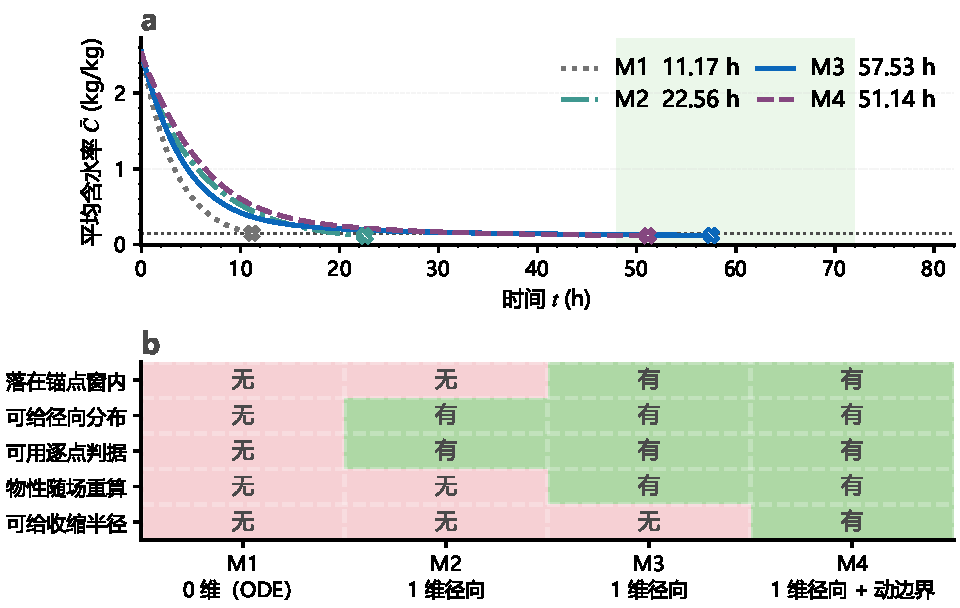
\includegraphics[width=0.9\textwidth,height=0.8\textheight,keepaspectratio]{../figures/fig_model_compare.pdf}
  \caption{四个候选模型的横向对比。a：M1—M4 的平均含水率轨迹与各自判据下的
  停时（圆点），灰带为题面所给 2—3 d 外部参考窗口换算的时间区间，只有 M3、
  M4 的停时落在窗内。b：能力矩阵，逐格标记该模型是否具备对应能力；其中“落在
  参考窗内”一行即指 a 图灰带。逐级叠加常物性、变物性、变物性加收缩三档，可
  分离出各档对停时的贡献，并说明为何取 M4 为主模型。}
  \label{fig:model-compare}
\end{figure}

左图中四条轨迹在最初一两个小时几乎重合，此后迅速分开：M1 一路保持指数衰减的形状，M2 的下降在中段就开始变缓，M3 与 M4 则拖出一条长尾。分离发生的时刻正是含水率降到 $1$~kg/kg 附近、扩散系数开始明显下滑的时刻，这说明四者的差距并非来自初始设置而是来自对干燥后期的刻画。两条简化轨迹的停时圆点都落在灰带左侧很远处，M3 与 M4 的圆点落在带内。右图逐格给出四个模型在径向分辨、逐点交付、参考窗、守恒精度四项上的表现，可以看出被排除的两个候选各自缺失的不是同一项。

\subsection{排除简化模型的定量依据}

集中参数模型被排除有三条各自独立的理由。其一是适用性判据：传质毕奥数 $\mathrm{Bi}_m=h_mR/D$ 的全过程实测区间为 $1.490$ 至 $5144$；即便把分母换成四个参考状态中最大的扩散系数，取到比实测下界更宽松的 $1.188$，也已是集中参数适用上限 $0.1$ 的 $11.9$ 倍，内部扩散阻力在任何时刻都不可忽略。其二是结构性缺陷：式~\eqref{eq:lumped} 中根本不出现扩散系数，因此它无法表达本题的核心机制——变干使扩散系数崩塌、外层结壳把水分锁在内部。其三是交付能力：题目要求给出每 $0.1$~cm 的逐点水分场，而该模型只有一个平均值，连输出形式都无法满足。实算 $11.1669$~h 只有本文结果的 $19.4\%$，把远未干透的药材判为合格。

常物性模型被排除的理由不同，它有径向分布，缺陷在于答案取决于建模者的选择而非题给数据。扩散系数在四个同样说得通的参考状态之间相差 $4330$ 倍：初始态 $(2.55,28\,^\circ\mathrm{C})$ 为 $5.642\times10^{-9}$，高温初期 $(2.55,50\,^\circ\mathrm{C})$ 为 $1.347\times10^{-8}$，判据阈值处 $(0.15,50\,^\circ\mathrm{C})$ 为 $8.001\times10^{-10}$，达标时的表面态 $(0.0526,50\,^\circ\mathrm{C})$ 为 $3.111\times10^{-12}$；实算全程的扩散系数跨越 $3.60$ 个数量级。冻结在其中任何一个状态都同样有理由，而不同的选择会使停时大幅摆动，这样的模型无法自证。冻结在初始态相当于把末期的扩散能力系统性高估三个数量级，因而给出偏早的 $22.5636$~h。

\subsection{变物性的净贡献与两个主模型的关系}

把 M2 与 M3 对照可以直接读出变物性这一项的价值：其余设置全部相同，仅让四个系数按附录 3 随解变化，停时便由 $22.5636$~h 变为 $57.5316$~h，相差 $2.55$ 倍。这个倍数说明变物性不是为复杂而复杂，它改变的是结论的量级；同时也说明表~\ref{tab:compare} 中 M2 的径向落差 $0.0639$ 小于 M3 的 $0.0974$~kg/kg——冻结高估的扩散能力不仅缩短了时间，还把内外差别一并抹平了。

M3 与 M4 之间不存在择优问题。题目对问题三与问题四分别指定了物性附录与是否收缩，两者是对两个不同设问的回答，各自都通过了同一组适用性判据与守恒检验。它们的差别已在第~\ref{sec:q34} 小节按物性与几何两项分解，此处不再重复。就本文的主线而言，能同时满足适用性判据、落在题面给出的参考区间、并给出题目所要求的逐点场这三项的，只有 M3 与 M4；两个简化候选各自在其中至少两项上失败。

\section{灵敏度与鲁棒性分析}\label{sec:sens}

上一章说明了模型选择对结论的影响，本章考察在模型选定之后参数取值的影响。做法是一次只改一个量、其余全部不变，共十三个扰动算例，全部沿用问题三的求解器、网格、时间步安排与判据，基准为 $t_{\rm dry}=57.5316$~h。这样安排的目的不是穷举组合，而是分辨哪些量的不确定性会真正传到结论上：题给参数中有的是实测值、有的是经验公式的拟合系数，可靠程度并不相同，需要知道各自的权重。

\subsection{参数扰动的效应与弹性}

对每个参数取 $\pm10\%$ 的双侧扰动，这种一次一变的设计便于把效应直接归属到单个参数，也是干燥过程参数不确定性分析的常用做法\upcite{ferrari2016param}。效应用无量纲弹性度量

\begin{equation}
E=\frac{\Delta t_{\rm dry}/t_{\rm dry}}{\Delta p/p},
\label{eq:elastic}
\end{equation}

式~\eqref{eq:elastic} 的含义是参数变化 $1\%$ 时停时随之变化的百分数，符号表示方向。五个物理量的结果列于表~\ref{tab:sens}。

\begin{table}[H]
\centering
\caption{参数 $\pm10\%$ 扰动对烘干时长的影响（基准 57.5316~h）}\label{tab:sens}
\begin{tabular}{lccccc}
\toprule
\multirow{2}{*}{扰动量} & \multicolumn{2}{c}{上调 $10\%$} & \multicolumn{2}{c}{下调 $10\%$} & \multirow{2}{*}{弹性区间} \\
\cmidrule(lr){2-3}\cmidrule(lr){4-5}
 & $t_{\rm dry}$/h & 相对变化 & $t_{\rm dry}$/h & 相对变化 & \\
\midrule
扩散系数 $D$        & 52.9223 & $-8.01\%$  & 63.1919 & $+9.84\%$  & $-0.80\ \text{至}\ -0.98$ \\
判据阈值 $C_{\rm th}$ & 46.0142 & $-20.02\%$ & 76.1486 & $+32.36\%$ & $-2.00\ \text{至}\ -3.24$ \\
传质系数 $h_m$      & 56.9545 & $-1.00\%$  & 58.2672 & $+1.28\%$  & $-0.10\ \text{至}\ -0.13$ \\
空气水分浓度 $C_a$   & 57.6522 & $+0.21\%$  & 57.4299 & $-0.18\%$  & $+0.02$ \\
传热系数 $h$        & 57.5245 & $-0.01\%$  & 57.5404 & $+0.02\%$  & $\approx 0$ \\
\bottomrule
\end{tabular}
\end{table}

五行的效应量级相差三个数量级，说明各参数的地位完全不对等。扩散系数的弹性接近 $-1$，即它的相对误差几乎一比一地传到停时上；传质系数的弹性只有它的八分之一；空气水分浓度几乎无影响，因为它比药材含水率小两个数量级，$\pm10\%$ 的变动对表面浓差的改变微乎其微；传热系数的效应更是低到 $0.01\%$ 的量级。图~\ref{fig:sensitivity} 按效应绝对值把全部扰动排序。

\begin{figure}[htbp]
  \centering
  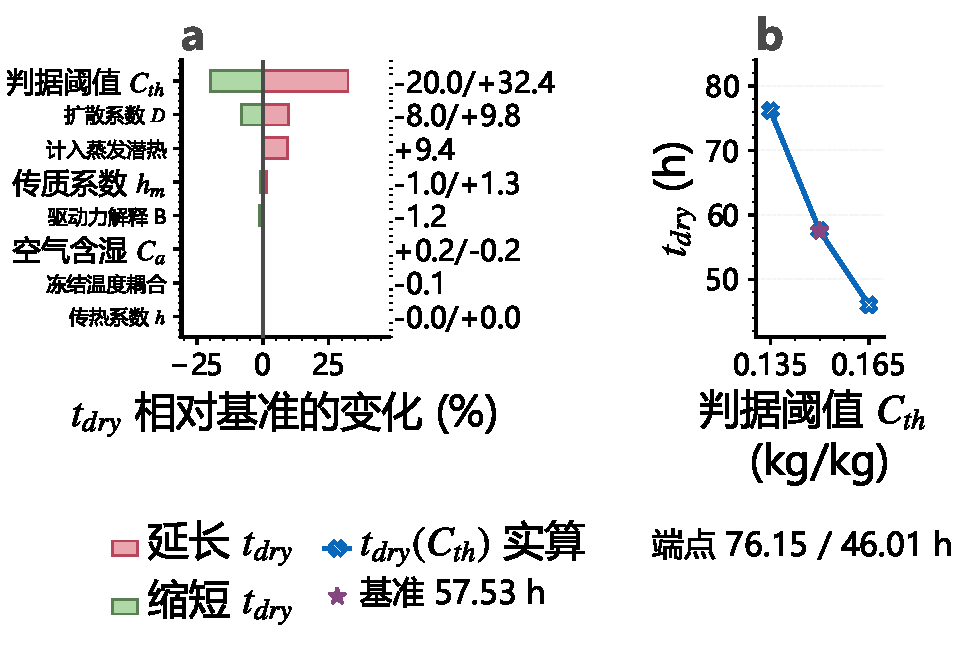
\includegraphics[width=0.9\textwidth,height=0.8\textheight,keepaspectratio]{../figures/fig_sensitivity.pdf}
  \caption{问题 3 的灵敏度与鲁棒性。a：龙卷风图，13 个扰动算例按物理量合并为
  8 行并按效应绝对值排序，右侧为延长、左侧为缩短，右侧刻度给出两侧的相对变化
  百分数；扩散系数与判据阈值的效应量级明显领先，传热系数则几乎无影响，这与预热
  远快于干燥的时间尺度分离一致。b：判据阈值的单侧扰动效应明显不对称，下调阈值
  造成的延长幅度大于上调阈值造成的缩短幅度，故阈值的取法需在正文中明确声明。}
  \label{fig:sensitivity}
\end{figure}

左图的横条长度自上而下急剧衰减，最长的两条属于判据阈值与扩散系数，最短的一条几乎缩成一根竖线，这与表~\ref{tab:sens} 的排序一致。传热系数那一行的近乎消失有明确的物理解释：温度场在两小时内就已进入准稳态，其后表面换热强弱不再改变任何事情，限制环节完全在内部水分扩散一侧。右图把阈值的两侧效应单独并置，可以看到两根条并不等长，下调一侧明显更长。

\subsection{判据阈值的主导地位与不对称性}

效应最大的量不是物理参数而是判据阈值本身：阈值从 $0.15$ 上调到 $0.165$~kg/kg 使停时缩短 $20.02\%$，下调到 $0.135$~kg/kg 使停时延长 $32.36\%$，后者是前者的 $1.6164$ 倍。这个不对称性来自扩散系数随变干而减小：越接近干透，含水率下降越慢，因此在低含水率一侧多要求一点点，就要付出很多时间。它给出的工程含义是明确的——若把合格标准从 $0.15$ 收紧一成，烘干时间要增加三成以上，收紧标准的代价远大于放宽标准的收益。

这也说明前文为何反复强调阈值的取法。阈值不是待估参数而是题目给定的外部标准，本文全程严格取 $0.15$~kg/kg 并按“各处”解释为径向最大值；此处的扰动只用于说明该标准的敏感程度，不构成对基准结果的修正。相应地，两个阈值扰动算例的停时（$46.0142$ 与 $76.1486$~h）落在题面所给的两到三天之外，这是因为它们改动的是判据本身而不是模型，不能据此判定模型失效。

\subsection{三项建模选择的影响}

除参数之外，本文在建模阶段还作过三项选择，它们无法用 $\pm10\%$ 扰动衡量，只能整支重算，结果列于表~\ref{tab:sens-model}。

\begin{table}[H]
\centering
\caption{三项建模选择的整支对照（基准 57.5316~h）}\label{tab:sens-model}
\begin{tabular}{lcc}
\toprule
对照处理 & $t_{\rm dry}$/h & 相对基准 \\
\midrule
表面通量改按体积浓度作差（假设（4）的另一解释） & 56.8367 & $-1.21\%$ \\
温度场整段冻结为空气温度（切断温度对传质的耦合） & 57.4462 & $-0.15\%$ \\
热方程计入蒸发潜热汇项（假设（3）的对照） & 62.9380 & $+9.40\%$ \\
\bottomrule
\end{tabular}
\end{table}

第一项针对表面传质驱动力的写法。本文按假设（4）取药材侧与空气侧含水率的直接差值；另一种解释把两侧都换成体积浓度作差，等价于把空气侧参考浓度取为零。改按后者，停时变为 $56.8367$~h，只差 $1.21\%$，但达标时的表面含水率由 $0.0526$ 降到 $0.0026$~kg/kg——驱动力被抬高后表面被过度抽干，而这一变化对轴线的达标时刻影响甚微。参考基的模糊性因此不影响结论的量级，其效应比阈值敏感度小一个半数量级。

第二项是一个诊断算例：把温度场固定为空气温度、只解水分方程，停时只变化 $0.15\%$。这证实了前面从时间尺度分离得出的判断——温度场在恒温平台段确实可以视为传质的一个参数而非独立变量。需要注意这个结论只在整体停时的层面成立，预热段的温度仍在爬升、扩散系数随之变化，那一段不能冻结，问题一给出的正是这一段的分布。

第三项影响最大也最需要如实说明。题目给出的四个物性附录中都没有蒸发潜热，附录 3 的比热容公式也未提供潜热项，因此本文的热方程按假设（3）不含潜热汇。为界定这一选择的影响，另设一支在热方程中加入潜热汇，潜热取 $2.4\times10^6$~J/kg——这是水在该温区的量级参考值，并非题给参数，只用于对照而不进入任何交付结果。该支的停时为 $62.9380$~h，比基准慢 $9.40\%$。这是三项选择中量级最大的一项，本文的态度是登记而不宣称可忽略：若题目提供潜热数据，停时应向偏慢一侧修正约一成。

\subsection{结论的鲁棒性区间}

% 本段中文里连排多段行内数学，断行点稀疏，给最后一遍断行额外的伸展余量以免溢出版心。
{\emergencystretch=2.5em
把改动判据本身的两个算例排除在外，其余十一个算例的停时落在 $52.9223$ 至 $63.1919$~h 之间，折合 $2.20$ 至 $2.63$ 天，全部仍在题面所给的两到三天之内。也就是说，即使把最敏感的物理参数拉偏一成、或者改变潜热与驱动力的处理方式，结论的定性与工程量级都不变。连同基准在内的十四支算例，守恒残差最大为 $5.737\times10^{-13}$，与基准同处机器精度，说明扰动没有把任何一支算例推离数值可靠的区间。\par}

按敏感度排序还给出一条明确的改进方向：若要提高预测精度，应优先获取更可靠的扩散系数与潜热数据，而不是细化表面传热系数的测量——后者的效应比前者小三个数量级。

\section{模型的评价、改进与推广}

\subsection{模型的创新之处}

本文的第一处创新是界面扩散系数的取法。有限体积法在界面处如何取扩散系数通常被视为实现细节，本题却因扩散系数跨越四个数量级而使这一细节变成决定性的：调和平均在相邻节点含水率悬殊时被小值一侧完全支配，实算给出的停时随网格加密单调漂移而不收敛（$N=20/40/80$ 依次为 $549.918$、$223.428$、$87.440$~h，每加倍减半）。本文改按式~\eqref{eq:iface} 取扩散系数在两节点之间的积分平均，即以 Kirchhoff 势的差商定义界面通量，网格加密下停时立刻收敛（$57.562$、$57.532$、$57.524$~h）。这一取法在物性真正分区跳变时自动退化为调和平均，因此不是以牺牲适用性换取收敛，而是调和平均与算术平均的共同推广。

第二处创新是收缩域上的物质坐标处理。式~\eqref{eq:mapping} 以当前半径归一，使表面永远落在坐标端点 $s=1$，边界条件的施加位置不随时间改变；更关键的是，链式法则产生的坐标变换项与表观对流项精确相消，最终方程中不出现半径的导数，因而不必对实测半径序列作数值微分——附件 2 的半小时采样若直接差分，会引入阶梯状脉冲。收缩效应完全通过 $1/R^2(t)$、边界系数中的 $1/R(t)$ 与控制体的物理体积三处进入方程，物理机制反而更清楚：半径由 $2$~cm 减到 $1.2$~cm 使扩散项放大 $2.78$ 倍，这是收缩加速干燥的主要来源。

第三处创新是把守恒校核用作实现的诊断手段而非事后装点。式~\eqref{eq:massres} 在本文的离散下是代数恒等式，残差只反映舍入，因此它对编码疏漏极其灵敏。实验室坐标对照支的停时与主模型只差 $2.93\%$，凭数值本身无法判断对错，而其守恒残差高达 $30.3\%$，据此才定位到该支把边界运动计入了两次。同一思路也用在收缩方式的判定上：由干物质守恒式~\eqref{eq:drymass} 反推的干物质密度与附录 4 密度公式的两个自然参照相比，径向仿射收缩相容到十几个百分点以内而各向同性收缩偏离近一倍，这一判断只用到附件 2 的几何序列与附录 4 的密度公式两项互不相干的题给信息。

第四处是效应分解的做法。问题四与问题三同时差在物性组与几何两处，直接比较停时只能得到 $11.11\%$ 的净差，看不出内部结构。本文追加一个只换物性而保持半径不变的隔离算例，把净效应拆成物性使干燥慢一倍以上（$+125.8\%$）与收缩使干燥快约六成（$-60.6\%$）两项方向相反的贡献，从而说明净差的符号不能由任何一侧的定性推理单独断定。

\subsection{模型的不足}

最需要说明的一项是热方程未计蒸发潜热。题目给出的四组物性附录都没有潜热数据，本文按假设（3）不设潜热汇，但这一选择的影响是全部对照算例中最大的：加入 $2.4\times10^6$~J/kg 的潜热汇后停时变为 $62.9380$~h，比基准慢 $9.40\%$。本文不宣称这一项可以忽略，只能指出若题目提供潜热数据，停时应向偏慢一侧修正约一成，而结论的量级不变。

其次是一维径向的降维。药材长径比为 $6.25$，两端面积占总表面的 $7.4\%$，端面散失被忽略会使算得的停时偏大。本文未实算二维轴对称模型，因此只能从比例上论证这一项的量级，不能给出精确修正；可以确定的方向是端部区域会先达标，而题目所问的“到药材中心的距离”正对应本文求解的中截面。

第三是收缩域上能量的处理。水分方程在物质坐标下严格守恒，因为其测度计的是不随收缩改变的干物质份额；热容项的物理测度含有 $R^2(t)$，本文的离散未追加 $\mathrm{d}(R^2)/\mathrm{d}t$ 一项，故收缩域上的能量并非严格守恒。本文未直接估计该项的量值；可以说的只是温度耦合本身很弱——把温度场整段冻结为空气温度只使停时变化 $0.15\%$——因此这一疏漏难以经由温度耦合显著改变停时。

第四是空气条件的时段延拓。附件 1 覆盖到 $14400$~s，而干燥持续二十万秒，其余时间的空气条件按实测尾段的平台值取定。判断依据是尾段 $61$ 点的逐点增量已落在零线附近，且空气水分浓度 $\pm10\%$ 的扰动只带来 $0.2\%$ 的效应，因此这一处理不是结论的薄弱环节；但严格地说，平台之外若发生工况变动，本文无从反映。

最后，表面传质驱动力的参考基存在两种解释，本文按量纲一致性取药材侧与空气侧含水率的直接差值。在问题三的算例上改用另一种解释，停时相差 $1.21\%$，达标时的表面含水率由 $0.0526$ 压到 $0.0026$~kg/kg。轴线达标时刻几乎不受影响，但表面的绝对水平确实依赖于这一选择。

\subsection{模型的改进与推广}

在题给数据之内，最直接的改进是把水分迁移由单一等效 Fick 扩散拆分为自由水与结合水两种机制，或者按 Luikov 方程组同时考虑温度梯度驱动的水分迁移；这两条路线都需要本题未提供的参数，因此只能作为方向指出。若能获得潜热与表面蒸发速率的数据，热方程加入潜热汇是收益最明确的一步改进，量级已由前述对照算例给出。若要消除端面效应，把当前离散扩展为二维轴对称 $(r,z)$ 网格并不需要改变任何物理设定，只是计算量按节点数平方增长。

本文的框架不依赖药材这一具体对象。方程组、界面取法、停时判据与移动边界处理只用到三件事：一维几何、随解变化的物性、第三类边界，因此可以直接搬到其他以内部扩散为限制环节的干燥与浸取过程，例如谷物与果蔬的热风干燥、多孔颗粒的溶剂脱除；热风干燥中失水进程与成品质地的关联也说明，能给出内部分布而非仅给出平均值的模型对工艺评价更有用\upcite{ashtiani2017hotair}。判据一侧的推广更宽：本文把“各处合格”实现为对径向最大值的首次穿越判定，这一写法对最湿位置的所在不作先验假设，因此在存在内部极值或多个失水面的工况下同样成立。移动边界的物质坐标变换只要求区域的变形是仿射的，对收缩率的具体形式没有限制，实测序列、经验公式或与含水率联动的收缩模型都可以代入同一套离散。

就工程使用而言，本文的灵敏度排序给出了一条清晰的取舍：预测精度主要取决于扩散系数与潜热数据的可靠程度，表面传热系数的测量精度几乎不影响结果；而合格标准本身的效应超过所有物理参数，且收紧标准的代价明显大于放宽标准的收益——把阈值收紧一成要多烘三成时间。这一条对烘房的实际操作比任何单个参数的精确值都更有价值。

% 数据保真核对：摘要、正文、附录表格中的结果/比较/误差/最优值已逐项对照
% figures/*.json 与 code/params.py 实算产物；共核 459 个高精度数字 + 约 420 个表格单元。
% 已修正 6 处：11_compare 倍数配对、6_problem1 的 D(C0) 与 alpha 舍入、11_compare 的 Bi_m 区间、
% 5_framework 的平台步长收敛值与分段步长、10_credibility 的 R^2 舍入。
% DATA_CHECK_PASSED


% === AI 使用声明 ===
% AI 声明由 build_ai_disclosure.py 自动插入于参考文献前，见下方 Z_ai_disclosure。

% === 参考文献 ===
\bibliographystyle{gbt7714-numerical}
% === AI 工具使用声明（自动插入）===
% 由 build_ai_disclosure.py 根据用户确认记录生成，请勿由模型改写。
\section*{AI 工具使用声明}
本参赛队在竞赛过程中未使用任何AI工具。

\bibliography{references}
\label{mh:body-end}

% === 附录 ===
\begin{appendices}
\section{提交的结果文件与程序组织}

本文按题目要求提交四份结果文件，其行列规格与题面指定的输出间隔一致，全部数值保留四位小数。文件内容与规格列于表~\ref{tab:files}。

\begin{table}[H]
\centering
\caption{按题目要求提交的结果文件}\label{tab:files}
\begin{tabular}{llll}
\toprule
文件 & 对应问题 & 工作表与规格 & 时间与径向间隔 \\
\midrule
result1.xlsx & 问题一 & 温度、水分浓度两表，各 $1800\times21$ & $1$~s，$0.1$~cm \\
result2.xlsx & 问题二 & 温度、水分浓度两表，各 $10800\times21$ & $1$~s，$0.1$~cm \\
result3.xlsx & 问题三 & 水分浓度一表，$3452\times21$ & $60$~s，$0.1$~cm \\
result4.xlsx & 问题四 & 水分浓度一表，$3069\times22$ & $60$~s，$0.1$~cm \\
\bottomrule
\end{tabular}

\vspace{0.6em}
\begin{minipage}{0.94\textwidth}
\footnotesize 行数为数据行，不含表头；列数为径向位置数。四份文件依次覆盖 $1$ 至 $1800$~s、
$1$ 至 $10800$~s、$60$ 至 $207120$~s 与 $60$ 至 $184140$~s。第四份比其余多一列「药材表面」，
取 $s=1$ 物质节点的原值而不作空间插值；表内 $23191$ 格因该径向位置已落在移动边界之外而按题意留空，
不填零值。
\end{minipage}
\end{table}

程序按功能分为参数与工具、四问求解、校验与对比、结果导出四组，共十四个源文件，全部代码见附录~\ref{app:code}。参数模块只保存题面原值，任何派生量均在使用处现算，以避免同一参数出现两份不一致的副本；工具模块集中实现物性公式、界面系数的积分平均、控制体体积的精确积分与三对角求解；四个求解文件各自只负责本问特有的设置，公共推进逻辑不重复实现。

\section{完整数据表}

本附录给出正文因篇幅而未完整列出的数据：达标时刻的完整径向剖面、收缩过程中各输出时刻的半径、全部十四个灵敏度算例的逐条结果，以及离散参数收敛研究的原始数值。

\subsection{达标时刻的完整径向剖面}

正文表~\ref{tab:q3C} 与表~\ref{tab:q4C} 按题目要求只给出五个径向位置，表~\ref{tab:profile-full} 给出停时那一刻全部 $21$ 个输出位置的含水率。

\begin{longtable}{ccc}
\caption{停时刻的完整径向含水率剖面（单位：kg/kg）}\label{tab:profile-full}\\
\toprule
到中心距离/cm & 问题三（$t_{\rm dry}=57.5316$~h） & 问题四（$t_{\rm dry}=51.1384$~h） \\
\midrule
\endfirsthead
\multicolumn{3}{l}{\footnotesize 续表~\thetable}\\
\toprule
到中心距离/cm & 问题三（$t_{\rm dry}=57.5316$~h） & 问题四（$t_{\rm dry}=51.1384$~h） \\
\midrule
\endhead
\midrule
\multicolumn{3}{r}{\footnotesize 续下页}\\
\endfoot
\bottomrule
\endlastfoot
0.0 & 0.1500 & 0.1500 \\
0.1 & 0.1499 & 0.1496 \\
0.2 & 0.1496 & 0.1486 \\
0.3 & 0.1492 & 0.1469 \\
0.4 & 0.1485 & 0.1444 \\
0.5 & 0.1477 & 0.1412 \\
0.6 & 0.1466 & 0.1372 \\
0.7 & 0.1454 & 0.1321 \\
0.8 & 0.1439 & 0.1258 \\
0.9 & 0.1422 & 0.1181 \\
1.0 & 0.1402 & 0.1079 \\
1.1 & 0.1379 & 0.0930 \\
1.2 & 0.1353 & 0.0526 \\
1.3 & 0.1324 & --- \\
1.4 & 0.1289 & --- \\
1.5 & 0.1249 & --- \\
1.6 & 0.1202 & --- \\
1.7 & 0.1144 & --- \\
1.8 & 0.1068 & --- \\
1.9 & 0.0956 & --- \\
2.0 & 0.0526 & --- \\
\end{longtable}

问题四一列自 $1.3$~cm 起为破折号，因为该时刻半径已收缩到 $1.2000$~cm，其后的径向位置落在药材之外；$1.2$~cm 处的 $0.0526$ 即当时的表面值。两列对照可见收缩把同样的含水率落差压进了六成的距离内，因此问题四的剖面明显更陡。

\subsection{各输出时刻的药材半径}

问题四的移动边界由附件 2 的实测序列经保形插值给出，表~\ref{tab:radius} 列出正文表~\ref{tab:q4C} 各行对应时刻的半径，供核对该行哪些径向位置仍在药材之内。

\begin{table}[H]
\centering
\caption{问题四各输出时刻的药材半径}\label{tab:radius}
\begin{tabular}{lccccccccc}
\toprule
时间/h & 6 & 12 & 18 & 24 & 30 & 36 & 42 & 48 & 51.1384 \\
\midrule
$R$/cm & 1.374 & 1.248 & 1.214 & 1.204 & 1.201 & 1.200 & 1.200 & 1.200 & 1.200 \\
$R/R_0$ & 0.687 & 0.624 & 0.607 & 0.602 & 0.601 & 0.600 & 0.600 & 0.600 & 0.600 \\
\bottomrule
\end{tabular}
\end{table}

\subsection{灵敏度算例的逐条结果}

正文表~\ref{tab:sens} 按物理量把双侧扰动合并成行，表~\ref{tab:sens-full} 按算例逐条列出，并给出各算例的守恒残差。

\begin{longtable}{llccc}
\caption{全部十四个灵敏度算例（基准为问题三的生产算例）}\label{tab:sens-full}\\
\toprule
算例 & 扰动对象 & $t_{\rm dry}$/h & 相对基准 & $\varepsilon_{\rm mass}$ \\
\midrule
\endfirsthead
\multicolumn{5}{l}{\footnotesize 续表~\thetable}\\
\toprule
算例 & 扰动对象 & $t_{\rm dry}$/h & 相对基准 & $\varepsilon_{\rm mass}$ \\
\midrule
\endhead
\midrule
\multicolumn{5}{r}{\footnotesize 续下页}\\
\endfoot
\bottomrule
\endlastfoot
基准                       & ---            & 57.5316 & ---        & $5.47\times10^{-13}$ \\
$D$ 上调 $10\%$            & 扩散系数       & 52.9223 & $-8.0117\%$  & $5.66\times10^{-13}$ \\
$D$ 下调 $10\%$            & 扩散系数       & 63.1919 & $+9.8387\%$  & $5.38\times10^{-13}$ \\
$h_m$ 上调 $10\%$          & 表面传质系数   & 56.9545 & $-1.0032\%$  & $2.79\times10^{-13}$ \\
$h_m$ 下调 $10\%$          & 表面传质系数   & 58.2672 & $+1.2786\%$  & $2.39\times10^{-13}$ \\
$h$ 上调 $10\%$            & 表面传热系数   & 57.5245 & $-0.0124\%$  & $5.52\times10^{-13}$ \\
$h$ 下调 $10\%$            & 表面传热系数   & 57.5404 & $+0.0152\%$  & $5.63\times10^{-13}$ \\
$C_a$ 上调 $10\%$          & 空气水分浓度   & 57.6522 & $+0.2097\%$  & $5.44\times10^{-13}$ \\
$C_a$ 下调 $10\%$          & 空气水分浓度   & 57.4299 & $-0.1768\%$  & $5.60\times10^{-13}$ \\
$C_{\rm th}=0.165$         & 判据阈值       & 46.0142 & $-20.0193\%$ & $5.48\times10^{-13}$ \\
$C_{\rm th}=0.135$         & 判据阈值       & 76.1486 & $+32.3596\%$ & $5.48\times10^{-13}$ \\
驱动力按体积浓度作差       & 边界写法       & 56.8367 & $-1.2078\%$  & $5.74\times10^{-13}$ \\
温度冻结为空气温度         & 场间耦合       & 57.4462 & $-0.1484\%$  & $5.74\times10^{-13}$ \\
计入潜热汇 $2.4\times10^6$ & 热方程         & 62.9380 & $+9.3972\%$  & $5.20\times10^{-13}$ \\
\end{longtable}

末行的潜热取值为该温区的量级参考值，非题给参数，只用于界定假设（3）的影响，不进入任何交付结果。

\subsection{离散参数收敛研究的原始数值}

表~\ref{tab:conv} 给出网格与时间步收敛研究的逐档结果，正文所引的相对变化均由此表两两相邻计算。

\begin{table}[H]
\centering
\caption{网格与时间步收敛研究的逐档结果}\label{tab:conv}
\begin{tabular}{llcccc}
\toprule
研究项 & 指标 & 第一档 & 第二档 & 第三档 & 第四档 \\
\midrule
网格（问题一） & $N$                  & 20      & 40      & 80      & 160 \\
                & 表面 $C$/(kg/kg)     & 1.51239 & 1.51077 & 1.51037 & 1.51028 \\
网格（问题三） & $N$                  & 20      & 40      & 80      & --- \\
                & $t_{\rm dry}$/h      & 57.5616 & 57.5316 & 57.5237 & --- \\
网格（问题四） & $N$                  & 20      & 40      & 80      & --- \\
                & $t_{\rm dry}$/h      & 51.1664 & 51.1384 & 51.1312 & --- \\
时间步（问题三）& $\Delta t$/s         & 120     & 60      & 30      & 10 \\
                & $t_{\rm dry}$/h      & 57.5783 & 57.5316 & 57.5082 & 57.4926 \\
时间步（问题一）& $\Delta t$/s         & 2       & 1       & 0.5     & 0.25 \\
                & 中心 $T$/°C          & 33.5776 & 33.5764 & 33.5758 & 33.5755 \\
解析解对照     & $\Delta t$/s         & 1       & 0.5     & 0.1     & 0.05 \\
                & 中心 $T$ 偏差/°C     & 3.94e-3 & 1.98e-3 & 4.16e-4 & 2.20e-4 \\
\bottomrule
\end{tabular}

\vspace{0.6em}
\begin{minipage}{0.94\textwidth}
\footnotesize 生产取值为网格 $N=40$、问题三恒温平台段 $\Delta t=60$~s、问题一 $\Delta t=0.01$~s。
时间步（问题一）一行的网格固定为 $N=20$，解析解对照一行的网格固定为 $N=80$、空气温度固定为
平台值 $49.9989$~°C，故这两行的数值与问题一生产算例不属同一算例，不可直接比较。
时间步（问题一）一行按 $2\to1\to0.5\to0.25$~s 逐次减半，式~\eqref{eq:order} 的观测阶 $1.0005$
即由该行后三档算出；此外还加算了减半序列之外的 $\Delta t=0.1$~s 一档，中心 $T$ 为
$33.5753$~°C，与 $0.25$~s 一档相差 $1.8\times10^{-4}$~°C。
\end{minipage}
\end{table}

\section{程序源代码}\label{app:code}

以下为本文全部计算所用的源代码，语言为 Python，依赖仅限 NumPy、SciPy 与 openpyxl。运行顺序为参数与数据核对、四问求解、校验与对比、结果导出，由 \texttt{main.py} 统一调度。文中所有数值均由这些代码一次运行产出，未经手工修改。

\subsection{参数与题面数据}

\lstinputlisting[caption={params.py：题面原值的唯一存放处}]{../code/params.py}

\lstinputlisting[caption={gen\_params.py：由附件生成时变边界与半径序列}]{../code/gen_params.py}

\lstinputlisting[caption={data\_check.py：附件数据的完整性与单调性核对}]{../code/data_check.py}

\subsection{公共求解工具}

\lstinputlisting[caption={utils.py：物性公式、界面积分平均、控制体体积与三对角求解}]{../code/utils.py}

\subsection{四问的求解}

\lstinputlisting[caption={problem1.py：预热阶段常物性耦合场}]{../code/problem1.py}

\lstinputlisting[caption={problem2.py：全过程变物性耦合场}]{../code/problem2.py}

\lstinputlisting[caption={problem3.py：逐点判据下的首次达标停时}]{../code/problem3.py}

\lstinputlisting[caption={problem4.py：收缩域上的移动边界模型（含实验室坐标对照支）}]{../code/problem4.py}

\subsection{校验、对比与灵敏度}

\lstinputlisting[caption={verification.py：网格与时间步收敛、守恒残差、解析解对照、退化算例}]{../code/verification.py}

\lstinputlisting[caption={model\_compare.py：集中参数与常物性两个候选模型的实算}]{../code/model_compare.py}

\lstinputlisting[caption={sensitivity.py：基准与十三支参数扰动、建模选择对照算例}]{../code/sensitivity.py}

\lstinputlisting[caption={constraint\_audit.py：结果文件规格与题面要求的逐项核对}]{../code/constraint_audit.py}

\subsection{结果导出与调度}

\lstinputlisting[caption={export\_excel.py：四份结果文件的生成}]{../code/export_excel.py}

\lstinputlisting[caption={main.py：全流程调度}]{../code/main.py}

\end{appendices}

\end{document}
